% ============================================================================
%  RELATÓRIO DE IMERSÃO \textemdash{} GRUPO 02 \textperiodcentered{} REVESTU
%  ODS 12: Consumo e Produção Sustentável
%  Projeto Integrador I / Design Thinking \textemdash{} Módulo 1, Turma A
%  ETE Cícero Dias
%
%  Compilação: pdflatex (2x) \textemdash{} compatível com Overleaf e Google Colab.
%  Estrutura no padrão de template da disciplina (capa, folha de rosto,
%  aberturas de seção numeradas, gráficos vetoriais e referências).
% ============================================================================

\documentclass[12pt, a4paper]{article}

% ---------- Codificação e idioma ----------
\usepackage[utf8]{inputenc}
\usepackage[T1]{fontenc}
\usepackage[portuguese]{babel}
\usepackage[margin=2.5cm]{geometry}
\setlength{\headheight}{15pt}   % evita aviso do fancyhdr

% ---------- Tipografia ----------
\usepackage{lmodern}
\usepackage{helvet}            % família sans (Helvetica) p/ títulos e capa
\renewcommand{\familydefault}{\rmdefault}

% ---------- Recursos gráficos e tabelas ----------
\usepackage{graphicx}
\usepackage{tabularx}
\usepackage{xltabular}    % tabularx que quebra entre páginas (matrizes)
\usepackage{booktabs}
\usepackage{array}
\usepackage{enumitem}
\usepackage{float}
\usepackage{caption}
\usepackage{framed}     % barra lateral dos destaques (estilo acadêmico)
\usepackage{lettrine}   % capitular (drop cap) no resumo, estilo livro
\usepackage{ragged2e}

% ---------- Cores e gráficos vetoriais ----------
\usepackage{xcolor}
\usepackage{colortbl}
\usepackage{pgfplots}
\usepackage{pgf-pie}
\pgfplotsset{compat=1.18}

% ---------- Layout de página, capa e títulos ----------
\usepackage{tikz}
\usetikzlibrary{shadows}
\usepackage{eso-pic}
\usepackage{titlesec}
\usepackage{fancyhdr}
\usepackage{xurl}
\usepackage{hyperref}

% ============================================================================
%  PALETA DO PROJETO  (extraída da persona "Flademir" \textemdash{} verde-oliva + amarelo)
%  >>> Para trocar a identidade visual, ajuste APENAS as 8 cores abaixo. <<<
% ============================================================================
\definecolor{oliveDeep}{HTML}{4F5715}   % oliva escuro \textemdash{} títulos e contraste
\definecolor{olive}{HTML}{6E7524}        % oliva principal \textemdash{} capa e cabeçalhos
\definecolor{oliveSoft}{HTML}{A9B24A}    % oliva claro \textemdash{} números e detalhes
\definecolor{accentYellow}{HTML}{E0C13C} % amarelo (post-it) \textemdash{} destaques
\definecolor{cream}{HTML}{F4F3E2}        % creme \textemdash{} fundos de bloco
\definecolor{creamMid}{HTML}{E6E7CC}     % creme médio \textemdash{} linhas de tabela
\definecolor{ink}{HTML}{1C1C18}          % quase-preto \textemdash{} texto
\definecolor{slate}{HTML}{555555}        % cinza \textemdash{} rótulos e dados
\definecolor{corCorrecao}{HTML}{B02A26}  % vermelho \textemdash{} anotações de correção
\definecolor{corCorrecaoBg}{HTML}{FAEDEC}% fundo claro das correções

% ---------- Hyperlinks ----------
\hypersetup{
    colorlinks=true,
    linkcolor=oliveDeep,
    filecolor=oliveDeep,
    urlcolor=olive,
    citecolor=olive,
    breaklinks=true
}

% ============================================================================
%  DADOS DO TRABALHO  (centralize aqui qualquer alteração de identificação)
% ============================================================================
\newcommand{\projTitulo}{REVESTU}
\newcommand{\projSubtitulo}{Solução para consumo consciente e reciclagem de vestuário}
\newcommand{\projODS}{ODS 12 \textemdash{} Consumo e Produção Sustentável}
\newcommand{\projGrupo}{Grupo 02}
\newcommand{\projIntegrantes}{Andréa \and Arthur Borges \and Luiz Henrique \and Matheus \and Yasmin}
\newcommand{\projCurso}{Técnico em Desenvolvimento de Sistemas}
\newcommand{\projModulo}{Módulo 1 \textbullet\ Turma A}
\newcommand{\projDisciplina}{Design Thinking \textbullet\ Projeto Integrador I}
\newcommand{\projProfessora}{Profa. Samara Silvia Sabino}
\newcommand{\projInstituicao}{ETE Cícero Dias}
\newcommand{\projEtapa}{Memorial de Projeto}
\newcommand{\projData}{Recife, Maio de 2026}

% ---------- Marca da escola (cabeçalho/capa) ----------
% Quando tiver a imagem da escola, salve-a como  imgs/logo-escola.png
% e troque a definição abaixo por:
%   \newcommand{\logoEscolaClara}{\includegraphics[height=1.1cm]{imgs/logo-escola-branca.png}}
%   \newcommand{\logoEscolaEscura}{\includegraphics[height=1.1cm]{imgs/logo-escola.png}}
\newcommand{\logoEscolaClara}{\textcolor{white}{\sffamily\bfseries\large ETE CÍCERO DIAS}}
\newcommand{\logoEscolaEscura}{\textcolor{oliveDeep}{\sffamily\bfseries\large ETE CÍCERO DIAS}}
\newcommand{\logoETE}{
\includegraphics[height=1.5cm]{imgs/logoETE.png}}
\newcommand{\logoNAVE}{
\includegraphics[height=1.5cm]{imgs/logoNAVE.png}}

% ============================================================================
%  ESTILO DAS ABERTURAS DE SEÇÃO  (número grande + título \textemdash{} estilo capítulo)
% ============================================================================
\titleformat{\section}[display]
  {\normalfont\sffamily}
  {\flushright\fontsize{84}{84}\selectfont\bfseries\color{oliveSoft}\thesection}
  {6pt}
  {\Huge\bfseries\color{oliveDeep}\filright}
\titlespacing*{\section}{0pt}{0pt}{30pt}

\titleformat{\subsection}
  {\normalfont\sffamily\large\bfseries\color{oliveDeep}}
  {\thesubsection}{0.6em}{}
\titlespacing*{\subsection}{0pt}{16pt}{6pt}

% Cada seção principal começa em página nova, com mais respiro no topo
\newcommand{\novaSecao}[1]{\clearpage\vspace*{2.2cm}\section{#1}}

% ---------- Cabeçalho e rodapé ----------
\fancypagestyle{corpo}{%
  \fancyhf{}
  \renewcommand{\headrulewidth}{0.6pt}
  \renewcommand{\headrule}{\hbox to\headwidth{\color{olive}\leaders\hrule height \headrulewidth\hfill}}
  \fancyhead[L]{\footnotesize\sffamily\textcolor{oliveDeep}{\textbf{REVESTU}}\ \textcolor{slate}{\textperiodcentered\ \projInstituicao}}
  \fancyhead[R]{\footnotesize\sffamily\textcolor{slate}{Memorial de Projeto \textperiodcentered\ Design Thinking}}
  \fancyfoot[L]{\footnotesize\sffamily\textcolor{slate}{\projODS}}
  \fancyfoot[R]{\footnotesize\sffamily\textcolor{oliveDeep}{\textbf{\thepage}}}
}

% ---------- Citação em destaque (estilo acadêmico: recuo + barra lateral) ----------
\newenvironment{citacaoBox}{%
  \par\vspace{6pt}%
  \def\FrameCommand{{\color{oliveSoft}\vrule width 2pt}\hspace{12pt}}%
  \MakeFramed{\advance\hsize-\width\FrameRestore}%
  \small\itshape\color{ink}%
}{%
  \par\endMakeFramed\vspace{6pt}%
}
\newcommand{\citacaoDestaque}[2]{%
  \begin{citacaoBox}#1\par\vspace{4pt}%
    {\normalfont\footnotesize\color{slate}\hfill\textsc{\textemdash{}\,#2}}%
  \end{citacaoBox}%
}

% ---------- Anotação de correção da professora (vermelho; pode ligar/desligar) ----------
\newif\ifmostrarcorrecoes
\mostrarcorrecoestrue   % <<< troque para \mostrarcorrecoesfalse na versão final (some as correções)
\newcommand{\correcao}[1]{%
  \ifmostrarcorrecoes
    \par\vspace{6pt}\noindent
    \setlength{\fboxsep}{9pt}%
    \fcolorbox{corCorrecao}{corCorrecaoBg}{%
      \begin{minipage}{\dimexpr\linewidth-2\fboxsep-2\fboxrule\relax}
        {\sffamily\bfseries\footnotesize\color{corCorrecao}\textsf{CORREÇÃO \textemdash{} PROFA. SAMARA}}\par\vspace{3pt}
        {\normalfont\small\color{corCorrecao} #1}
      \end{minipage}}%
    \par\vspace{6pt}
  \fi
}

% Item de legenda de cores p/ gráficos (swatch + texto da resposta, intacto)
\newcommand{\swatch}[1]{\raisebox{0.5pt}{\tikz{\fill[#1] (0,0) rectangle (9pt,9pt);}}}
\newcommand{\legendaItem}[2]{%
  \noindent\swatch{#1}\hspace{6pt}\begin{minipage}[t]{\dimexpr\linewidth-18pt\relax}#2\end{minipage}\par\vspace{3pt}%
}

% Banner horizontal: imagem cortada em faixa (largura total, altura fixa)
\newcommand{\bannerImg}[2][5.6cm]{%
  \noindent\begin{tikzpicture}
    \clip (0,0) rectangle (\linewidth,#1);
    \node[anchor=center, inner sep=0] at (0.5\linewidth, 0.5*#1) {\includegraphics[width=\linewidth]{#2}};
    \draw[cream, line width=0.8pt] (0,0) rectangle (\linewidth,#1);
  \end{tikzpicture}\par
}

\setlength{\parskip}{6pt}
\setlength{\parindent}{0pt}

\begin{document}

% ============================================================================
%  CAPA  \textemdash{}  estilo bloco de cor (referência: capa University of Dundee)
% ============================================================================
\begin{titlepage}
\thispagestyle{empty}
\begin{tikzpicture}[remember picture, overlay]
  % --- Imagem de capa sangrando na página inteira ---
  \begin{scope}
    \clip (current page.south west) rectangle (current page.north east);
    \node at (current page.center) {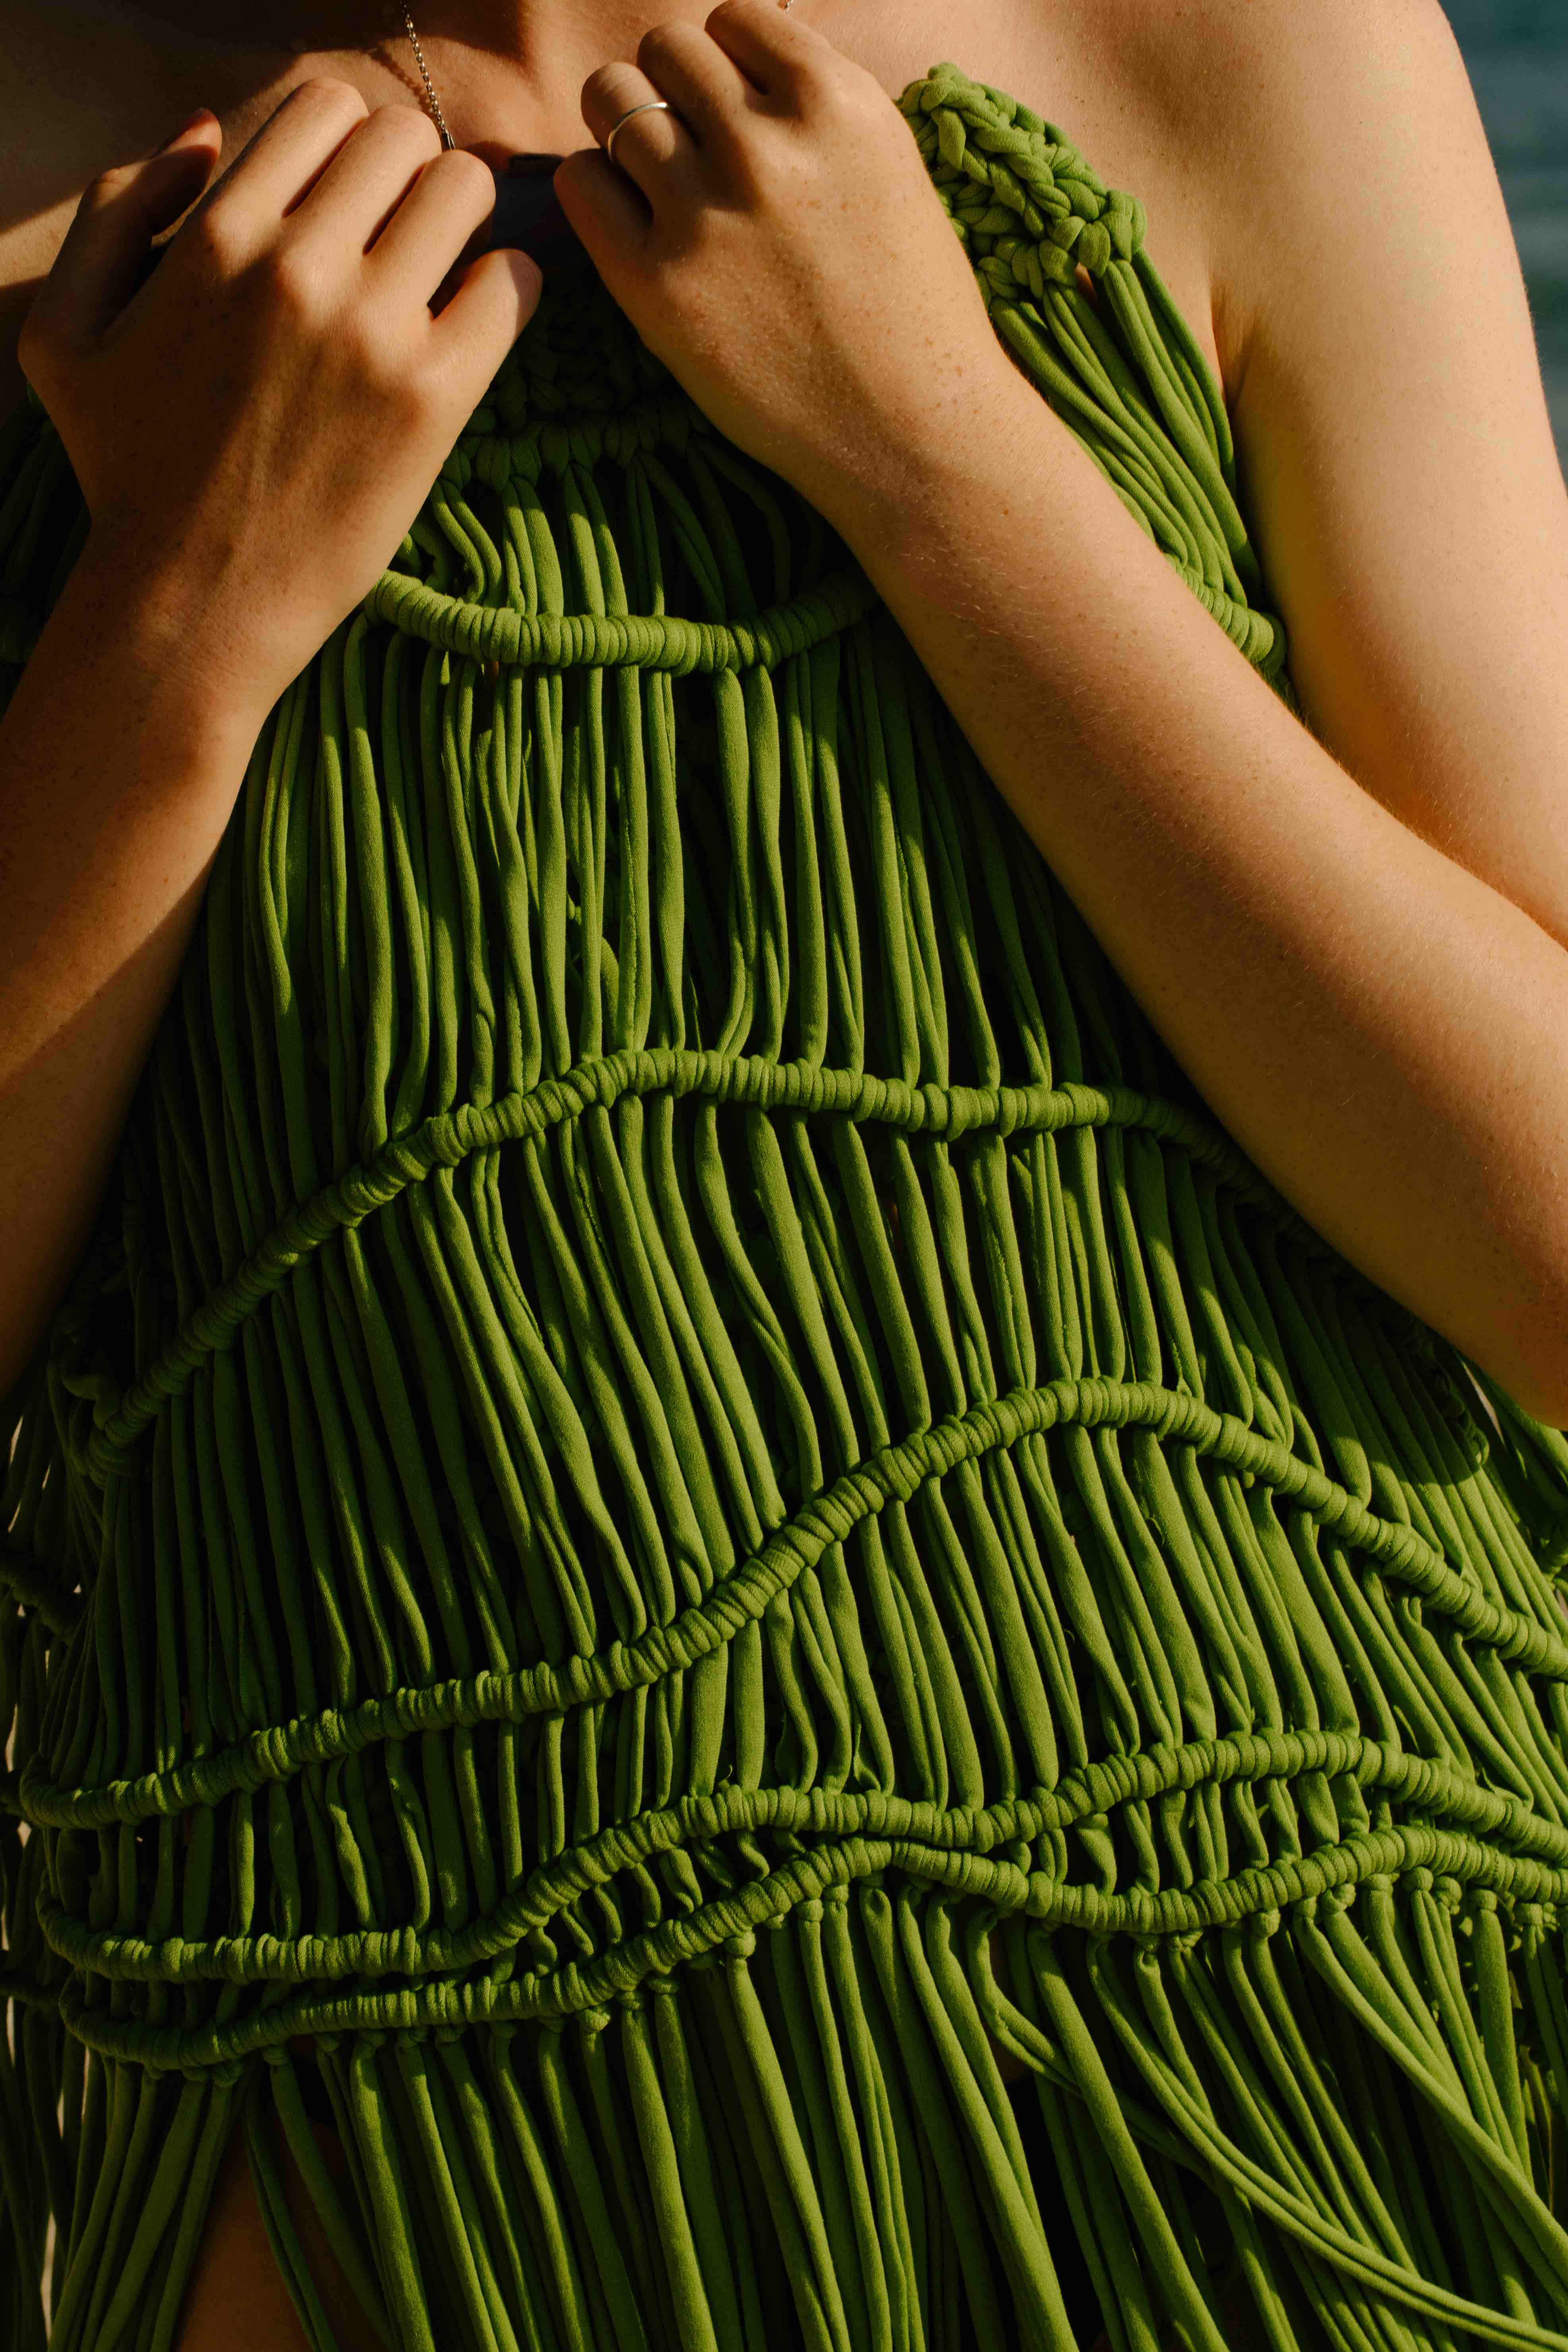
\includegraphics[width=\paperwidth]{imgs/capa.jpg}};
  \end{scope}

  % --- Escurecimento (degradê em camadas) para legibilidade ---
  \fill[black, opacity=0.20] (current page.south west) rectangle ([yshift=9.5cm]current page.south east);
  \fill[black, opacity=0.26] (current page.south west) rectangle ([yshift=6.0cm]current page.south east);
  \fill[black, opacity=0.40] (current page.south west) rectangle ([yshift=3.2cm]current page.south east);
  \fill[black, opacity=0.24] (current page.north west) rectangle ([yshift=-2.7cm]current page.north east);

  % --- Moldura fina (vibe livro) ---
  \draw[cream, line width=0.6pt]
    ([shift={(0.9cm,0.9cm)}]current page.south west)
    rectangle ([shift={(-0.9cm,-0.9cm)}]current page.north east);

  % --- Topo: instituição ---
  \node[anchor=north, text=cream, font=\sffamily] at ([yshift=-1.7cm]current page.north)
    {\small ETE CÍCERO DIAS \ \textbullet\ \ NAVE};

  % --- Bloco de título (terço inferior) ---
  \node[anchor=south west, text=white, align=left] at ([shift={(1.7cm,4.0cm)}]current page.south west)
    {\sffamily\bfseries\fontsize{82}{82}\selectfont REVESTU};
  \node[anchor=north west, text=cream, align=left, text width=15.5cm] at ([shift={(1.8cm,3.6cm)}]current page.south west)
    {\sffamily\large \projSubtitulo};

  % --- Linha + metadados ---
  \draw[cream!85, line width=0.5pt]
    ([shift={(1.8cm,2.75cm)}]current page.south west) -- ([shift={(9.0cm,2.75cm)}]current page.south west);
  \node[anchor=north west, text=cream, align=left] at ([shift={(1.8cm,2.55cm)}]current page.south west)
    {\sffamily\footnotesize MEMORIAL DE PROJETO \ \textbullet\ \ ODS 12 \ \textbullet\ \ GRUPO 02};

  % --- Crédito da foto (discreto) ---
  \node[anchor=south east, text=cream, opacity=0.75, font=\sffamily\tiny] at ([shift={(-1.1cm,1.1cm)}]current page.south east)
    {Foto: João Maraschin / divulgação};
\end{tikzpicture}
\end{titlepage}

% ============================================================================
%  FOLHA DE ROSTO  \textemdash{}  estilo minimalista (referência: EPFL)
% ============================================================================
\thispagestyle{empty}
\vspace*{2.2cm}
\begin{center}
  {\logoETE\hspace{1.4cm}\logoNAVE}\\[2.4cm]

  {\sffamily\footnotesize\color{slate} \MakeUppercase{\projODS}}\\[0.45cm]
  {\color{oliveSoft}\rule{2.4cm}{1.2pt}}\\[1.0cm]

  {\sffamily\bfseries\color{ink}\fontsize{56}{56}\selectfont \projTitulo}\\[0.55cm]
  {\itshape\large\color{oliveDeep} \projSubtitulo}\\[2.6cm]

  {\sffamily\color{slate}\large \projGrupo \quad\textperiodcentered\quad \projModulo}\\[0.55cm]
  {\color{ink} Andréa \ \textperiodcentered\ \ Arthur Borges \ \textperiodcentered\ \ Luiz Henrique \ \textperiodcentered\ \ Matheus \ \textperiodcentered\ \ Yasmin}
\end{center}

\vfill

\begin{center}
  {\color{oliveSoft}\rule{0.42\textwidth}{0.5pt}}\\[0.7cm]
  {\sffamily\footnotesize\color{slate}
    \projInstituicao \ \textbullet\ \ \projCurso\\[3pt]
    \projDisciplina\\[3pt]
    \projProfessora \quad\textperiodcentered\quad \projEtapa\\[3pt]
    \projData}
\end{center}
\vspace{1.2cm}

\clearpage

% ============================================================================
%  PÁGINA DA EQUIPE  \textemdash{}  um espaço de foto para cada integrante
% ============================================================================
\thispagestyle{empty}
\vspace*{1.5cm}
\begin{center}
  {\logoETE\hspace{1.4cm}\logoNAVE}\\[1.2cm]
  {\sffamily\bfseries\color{oliveDeep}\fontsize{34}{34}\selectfont \projTitulo}\\[0.25cm]
  {\sffamily\color{slate}\large Equipe \textbullet\ \projGrupo\ \textbullet\ \projModulo}\\[1.5cm]

  \newcommand{\membro}[1]{%
    \begin{minipage}[t]{3.7cm}\centering
      \setlength{\fboxsep}{0pt}%
      \fcolorbox{oliveSoft}{cream}{\parbox[c][4.7cm][c]{3.7cm}{\centering\color{slate}\scriptsize\itshape [ foto ]}}\\[6pt]
      {\sffamily\small\color{ink} #1}
    \end{minipage}}

  \membro{Andréa}\hspace{0.55cm}%
  \membro{Arthur Borges}\hspace{0.55cm}%
  \membro{Luiz Henrique}\\[0.95cm]
  \membro{Matheus}\hspace{0.55cm}%
  \membro{Yasmin}
\end{center}
\clearpage

% ============================================================================
%  PÁGINA DA PROFESSORA  \textemdash{}  o desafio + tempo + foto (recorrente)
%  >>> Texto genérico, reutilizável em todos os projetos.
%      Ajuste a duração em \duracaoProjeto abaixo.
% ============================================================================
\thispagestyle{empty}
\newcommand{\duracaoProjeto}{1º de abril a 1º de junho de 2026}   % <<< ajuste o período aqui
\vspace*{1.0cm}

{\centering\sffamily\footnotesize\color{olive} NOTA DA PROFESSORA\par}
\vspace{0.28cm}
{\centering\sffamily\bfseries\fontsize{36}{36}\selectfont\color{ink} O Desafio\par}
\vspace{0.28cm}
{\centering{\color{oliveSoft}\rule{2.6cm}{1.2pt}}\par}
\vspace{0.7cm}

\begin{center}
\begin{minipage}{0.82\textwidth}
{\centering\itshape\large\color{oliveDeep} Aprender resolvendo problemas reais: por que um desafio como este vale mais do que uma prova.\par}
\vspace{0.55cm}

\setlength{\parskip}{6pt}
\color{ink}
Este memorial documenta um \textbf{projeto integrador} conduzido pelo método do \textbf{Design Thinking}. Partindo de um dos Objetivos de Desenvolvimento Sustentável (ODS) da ONU, cada grupo identifica um problema real, investiga-o a fundo nas etapas de Imersão e Definição e chega à proposta de um protótipo. Não é um exercício teórico: é a vivência completa de como uma ideia se transforma em solução, conduzida ao longo de cerca de dois meses (\duracaoProjeto).

Do ponto de vista \textbf{pedagógico}, o desafio coloca o estudante no centro da própria aprendizagem. Em vez de receber respostas prontas, ele formula perguntas, coleta dados, erra, refaz e defende suas escolhas. Essa aprendizagem ativa desenvolve pensamento crítico, empatia com o usuário, trabalho em equipe e autonomia \textemdash{} competências que nenhuma prova tradicional consegue medir.

Do ponto de vista \textbf{mercadológico}, é exatamente assim que se trabalha no mundo real. Pesquisa de usuário, definição de problema, prototipação e validação são as etapas de qualquer time de produto, design ou tecnologia. Ao terminar, o estudante não leva apenas uma nota: leva um caso documentado, material de portfólio e a experiência concreta que o mercado procura.
\end{minipage}
\end{center}

\vfill

\begin{center}
  {\color{creamMid}\rule{0.35\textwidth}{0.6pt}}\\[0.5cm]
  \begin{tikzpicture}
    \node[circle, draw=oliveSoft, line width=1.5pt, minimum size=3.0cm, inner sep=0,
          path picture={\node at (path picture bounding box.center)
            {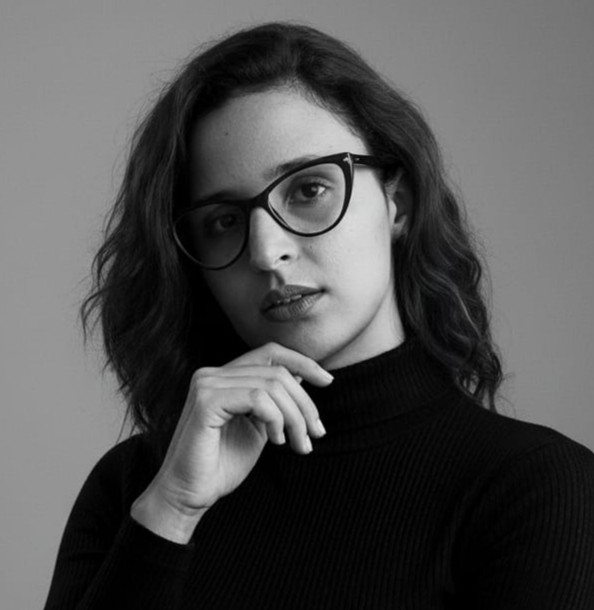
\includegraphics[width=3.3cm]{imgs/avatar-samara.jpg}};}] {};
  \end{tikzpicture}\\[0.4cm]
  {\sffamily\bfseries\color{oliveDeep} Profa. Samara Silvia Sabino}\\[3pt]
  {\sffamily\footnotesize\color{slate} Design Thinking \textperiodcentered\ Projeto Integrador \textperiodcentered\ ETE Cícero Dias}\\[2pt]
  {\sffamily\footnotesize\color{slate} \duracaoProjeto}
\end{center}
\vspace{0.9cm}
\clearpage

% ============================================================================
%  RESUMO \textperiodcentered{} PALAVRAS-CHAVE \textperiodcentered{} DESTAQUES
% ============================================================================
\pagestyle{corpo}

\begin{center}
  {\sffamily\large\color{oliveDeep} \MakeUppercase{Resumo}}\\[3pt]
  {\color{oliveSoft}\rule{1.8cm}{1pt}}
\end{center}
\vspace{0.5cm}

{\color{ink}
\lettrine[lines=3, lhang=0.08, findent=3pt, nindent=8pt]{\color{oliveDeep}\sffamily N}{osso} projeto busca entender como grandes marcas incentivam o consumo de seus artigos e produtos. Também buscamos saber como a o próprio site oferece os produtos que o usuário procura, será que o site induz o cliente de forma positiva? O ajudando em suas procuras ou apenas jogando informações e produtos que talvez não sejam o que ele procura? Incentivando assim o consumismo desenfreado\ldots\ Assim a ODS 12 se encaixaria totalmente na ideia de consumo, produção responsável e economia circular. Nossa plataforma seria um incentivo tanto para o consumidor quanto para grandes empresas. Durante nossa pesquisa e formulação da ideia, buscamos entender o real impacto que o descarte de artigos de vestiário causam em nosso ecossistema e quais são os caminhos para trazer um futuro mais sustentável e ecológico.
\par}

\vspace{6pt}
\noindent\textbf{Palavras-chave:} Reciclagem; Fast Fashion; Economia circular; Poliéster; Greenwashing; ACV (análise de ciclo de vida); Ecofashion; ODS 12.

\vspace{10pt}
\noindent{\sffamily\bfseries\color{oliveDeep} Destaques}
\vspace{2pt}

\begin{itemize}[leftmargin=1.2em, itemsep=4pt, label=\textcolor{oliveSoft}{\textbf{\textbullet}}]
  \item O setor têxtil é um dos mais poluentes do mundo: o fast fashion gera cerca de 92 milhões de toneladas de resíduos por ano.
  \item O poliéster e as fibras sintéticas predominam nas peças e dificultam a reciclagem.
  \item O greenwashing mascara práticas insustentáveis e confunde o consumidor.
  \item A principal barreira ao descarte correto é logística: faltam pontos de coleta e tempo.
  \item O público exige transparência sobre a durabilidade e o destino final das roupas.
\end{itemize}

\correcao{A estrutura geral do documento está incorreta. Revisar a ordem das seções seguindo o roteiro da disciplina (Imersão): a sequência das etapas e o encadeamento entre Pesquisa Desk, Observação e Formulário precisam ser reorganizados.}

% ============================================================================
%  SUMÁRIO
% ============================================================================
\clearpage
\vspace*{0.4cm}
{\sffamily\bfseries\fontsize{34}{34}\selectfont\color{oliveDeep} Sumário}\par
\vspace{4pt}{\color{olive}\rule{\linewidth}{1.5pt}}\par
\vspace{0.8cm}
\setcounter{tocdepth}{2}
\makeatletter
\@starttoc{toc}
\makeatother

% ============================================================================
%  1. INTRODUÇÃO
% ============================================================================
\clearpage
\bannerImg{imgs/intro.jpg}
\vspace{0.5cm}
\section{Introdução}

Para a criação do projeto foi necessário entender e usar o design thinking, ``uma abordagem criativa, que é centrada nas pessoas, com o objetivo na resolução de problemas e desenvolvimento de soluções inovadoras. O foco principal é entender as necessidades e desejos das pessoas, para quem um produto, serviço ou sistema está sendo projetado.

Esse processo de entendimento da percepção do usuário para desenho de protótipos com a finalidade de testes passa por divergências e convergências. O quer dizer isso: no design thinking são trabalhadas quatro etapas. A dica é `faça e refaça' quantas forem necessárias.''\textsuperscript{3}

Com isso, pensando na resolução de um tão problema real como: o destino dos resíduos gerados a partir do consumo de artigos de vestuário, pensamos em um produto digital (plataforma, aplicativo) para ajudar no consumo consciente e responsável, mas também do descarte correto (reciclagem).

Para dar mais sentido ao nosso projeto, conectamos ele com uma das ODS's da ONU. O que buscamos é que um problema real seja solucionado ou minimizado. A ODS escolhida foi a 12 que abrange o consumo e a produção responsável, e com nossa ideia vimos que as metas 12.2, 12.5 e 12.8 se relacionam com nossa ideia principal.

\clearpage
\subsection*{Metas da ODS 12}
\begin{itemize}[leftmargin=1.4cm, itemsep=10pt]
  \item[\textcolor{olive}{\textbf{12.2}}] Alcançar a gestão sustentável e o uso eficiente dos recursos naturais.

  \item[\textcolor{olive}{\textbf{12.5}}] Reduzir substancialmente a geração de resíduos por meio da prevenção, redução, reciclagem e reuso.
  \begin{itemize}[label=\textcolor{oliveSoft}{\textbullet}, leftmargin=1cm, topsep=4pt, itemsep=3pt]
    \item Podemos analisar se a marca produz de forma sustentável e se ela incentiva a economia circular para seus clientes.
    \item Nosso indução para as marcas terem cada vez mais produtos sustentáveis.
    \item Nossa ideia de incentivar a reciclagem em conjunto com as próprias marcas com os pontos de descarte.
  \end{itemize}

  \item[\textcolor{olive}{\textbf{12.8}}] Garantir que as pessoas, em todos os lugares, tenham informação relevante e conscientização para o desenvolvimento sustentável e estilos de vida em harmonia com a natureza.
  \begin{itemize}[label=\textcolor{oliveSoft}{\textbullet}, leftmargin=1cm, topsep=4pt, itemsep=3pt]
    \item Nossa plataforma seria esse meio para as pessoas acharem as informações sobre o que elas usam e como usar de forma mais consciente.
  \end{itemize}
\end{itemize}

\subsection*{O projeto na prática}
É uma ponte para a escolha dos clientes em um produto, talvez ele não compre na plataforma\ldots\ Mas pode ser uma ``rede social de avaliação e pesquisa'' e incentivo a sustentabilidade. A ideia é uma plataforma que tanto as marcas iam se cadastrar como os consumidores para um relacionamento entre ambos.

% ============================================================================
%  2. METODOLOGIA
% ============================================================================
\novaSecao{Metodologia}

\subsection{Matriz de Alinhamento}
Para garantir que o projeto estivesse focado no escopo e no desafio corretos, os parâmetros de alinhamento foram definidos da seguinte forma:

\renewcommand{\arraystretch}{1.45}
\begingroup
\small
\begin{xltabular}{\textwidth}{!{\color{oliveSoft}\vrule}>{\bfseries\color{oliveDeep}\raggedright\arraybackslash}p{4.1cm}!{\color{oliveSoft}\vrule}X!{\color{oliveSoft}\vrule}}
\arrayrulecolor{oliveSoft}\hline
\rowcolor{olive}\multicolumn{2}{!{\color{oliveSoft}\vrule}c!{\color{oliveSoft}\vrule}}{\textcolor{white}{\sffamily\bfseries IDENTIFICAÇÃO}}\\ \hline
Nome / Número do Grupo & Revestu / Grupo 02 \\ \hline
Integrantes & Yasmin, Matheus, Luiz Henrique, Arthur borges, Andréa. \\ \hline
ODS Escolhida & ODS 12, Produção e consumo responsável \\ \hline
\rowcolor{olive}\multicolumn{2}{!{\color{oliveSoft}\vrule}c!{\color{oliveSoft}\vrule}}{\textcolor{white}{\sffamily\bfseries IMERSÃO}}\\ \hline
Quem pode estar sendo afetado? & pessoas que moram perto de aterros, onde materiais de vestuario estão sendo descartados de forma errada. \\ \hline
O que o grupo quer descobrir? & com gerar na população um consumo consciente e ajudar os consumidores a praticarem o descarte correto de roupas, calçados etc. \\ \hline
Quais técnicas de imersão planejam usar? & pesquisa desk, questionario para saber com a população lia com o descarte de tais materiais e observação para entender como o material usado nos artigos afetam nosso dia dia e o planeta. \\ \hline
\rowcolor{olive}\multicolumn{2}{!{\color{oliveSoft}\vrule}c!{\color{oliveSoft}\vrule}}{\textcolor{white}{\sffamily\bfseries ESCOPO}}\\ \hline
O que está DENTRO do escopo? & direcionar e facilitar a reciclagem, interação e transparencia de marcas e garantir um consumo consciente e moderado. \\ \hline
O que está FORA do escopo? & Compras diretas na plataforma, criar pontos próprios de coleta. O intuito é um aplicativo para ajudar na escolha de artigos de vestimenta e direcionar o criente para o descarte correto após o fim do ciclo de vida de seu pertence. \\ \hline
Hipótese de solução (ideia inicial) & A criação de um aplicativo / rede social que permite que o publico e as marcas falem sobre os produtos e consomem e oferecem com informações de: ciclo de vida, uso ideal, como preservar e como reciclar. Assim gerando econômia circular e ajudando todos a fazerem compras conscientes e incentivando marcas a serem sustentáveis. \\ \hline
Resultado esperado da imersão & Permitir que usuários vejam tudo que o produto oferece, como e para qual situação ele é mais usual, como preservar produtos que já adquiriram e mostrar pontos de coleta daspróprias marcas para a permitir a reciclagem, e como bônus converter a reciclagem em pontos na loja / marca. \\ \hline
\end{xltabular}
\endgroup

\subsection{Matriz CSD}
Este quadro ajuda a visualizar o que o grupo já domina e tem certeza de como fazer, as suposições sobre tudo que engloba o projeto e as dúvidas que ainda restam \textemdash{} sendo estas últimas o guia principal da pesquisa de campo.

\renewcommand{\arraystretch}{1.4}
\begingroup
\small
\begin{xltabular}{\textwidth}{!{\color{oliveSoft}\vrule}X!{\color{oliveSoft}\vrule}X!{\color{oliveSoft}\vrule}X!{\color{oliveSoft}\vrule}}
\arrayrulecolor{oliveSoft}\hline
\rowcolor{olive}\multicolumn{3}{!{\color{oliveSoft}\vrule}c!{\color{oliveSoft}\vrule}}{\textcolor{white}{\sffamily\bfseries MATRIZ CSD \textemdash{} REVESTU}}\\ \hline
\rowcolor{creamMid}
\centering\textbf{CERTEZAS} & \centering\textbf{SUPOSIÇÕES} & \centering\arraybackslash\textbf{DÚVIDAS} \\
\rowcolor{cream}
\centering\footnotesize\textit{O que é fato ou base do projeto} & \centering\footnotesize\textit{O que achamos que é verdade, mas precisamos validar} & \centering\arraybackslash\footnotesize\textit{Perguntas que a Pesquisa Desk deve responder} \\ \hline
\endhead
A indústria têxtil (Fast Fashion) é uma das mais poluentes do mundo.
& As pessoas vão se dar ao trabalho de levar a roupa até um ponto de coleta por causa de pontos / descontos.
& Como funciona juridicamente a responsabilidade pelo descarte têxtil no Brasil? \\ \hline
Os consumidores têm dificuldade em saber como e onde descartar roupas velhas.
& As grandes multinacionais aceitarão se cadastrar em uma plataforma que permite avaliações negativas de durabilidade dos seus produtos.
& Existem tecnologias baratas (como QR Codes ou etiquetas inteligentes) para garantir que a peça foi realmente reciclada? \\ \hline
Roupas de poliéster e materiais sintéticos demoram centenas de anos para se decompor.
& Gamificação: rankings e selos (estilo Duolingo) são suficientes para mudar o hábito de descarte das pessoas.
& Qual é a média de desconto que as marcas estão dispostas a oferecer para incentivar a reciclagem? \\ \hline
Não existem muitas formas de consultar a duração de um produto antes de comprar e usá-lo.
& O usuário prefere responder um quiz de ``necessidades'' antes de ver os produtos.
& Como seria um ponto de coleta realmente fácil de acessar? Onde seria? Nas lojas, ou em pontos estratégicos como shoppings e grandes centros? \\ \hline
Marcas como O Boticário e C\&A já possuem algum nível de logística reversa.
& Produtos sustentáveis são percebidos pelo público como ``mais caros'' ou ``menos bonitos''.
& \\ \hline
\end{xltabular}
\endgroup

% ============================================================================
%  3. A PESQUISA DESK
% ============================================================================
\novaSecao{A Pesquisa Desk}

Nossa pesquisa teve como intuito de entender como o mercado e industrial da moda funcionam e como os materiais utilizados na fabricação podem ser reciclados de forma correta e eficaz.

Alguns dos temas e observações feitas durante a pesquisa foram essenciais para a idealização do projeto, assim como são importantes para a implementação.

O estudo sobre o materiais usados na fabricação das roupas diz muito sobre seu destino e como nosso propósito é a reciclagem exploramos essa temática. O fast fashion foi importante para entender a dinâmica entre consumo, produto e consumidor e por fim o estudo de marcas que usam Greenwashing nos mostra comportamentos que precisam ser melhorados em relação as marcas que fornecem esses materiais.

\correcao{Falta informar o escopo temporal da pesquisa: até quando (e a partir de quando) foram feitas as buscas no Google. Indicar o período de coleta dos dados/artigos consultados.}

\subsection{Poliéster: o tecido poluente}
A reciclagem de tecidos sintéticos é algo dificil de ser feito, se a coleta de tais fosse mais eficiente seriam um pouco mais fáceis de ser reciclado, mas é de estrema importância o uso de tecidos com material natural. Mesmo os principais métodos para a reciclagem de material têxtil tendo um alto custo e que requerer diversas etapas, é essencial para uma forma de auxiliar essa pratica que ajudará a sociedade a ter um consumo mais consciente e manter a produção desses artigos mais sustentável.

\citacaoDestaque{``A princípio esse tipo de reciclagem iria ajudar a reduzir a necessidade do consumo de materiais virgens e diminuiria a quantidade de tecidos que vão parar nos aterros, auxiliando na limitação do impacto no meio ambiente. Talvez futuramente teremos outras técnicas mais aprimoradas que irão baratear esse tipo de processo.''\textsuperscript{4}}{Reciclagem têxtil: algodão e poliéster}

\citacaoDestaque{``há sim possibilidade de reciclar os retalhos e transformá-los em uma nova peça, porém acaba não sendo o foco das indústrias nesses setores. Pois teriam de ter uma grande disponibilização de pessoas para fazer o processo de separação dos retalhos por cores e por composição, aumentando o custo do processo. Mesmo tendo isso como um fator complicador, as empresas que acatarem esse tipo de trabalho, com o tempo terá um baixo custo no processo pois não precisaria investir no plantio e em agrotóxicos que causam impacto no meio ambiente.''\textsuperscript{1}}{Reciclagem têxtil}

\subsection{Fast fashion}
O fenômeno do fast fashion revolucionou a indústria global ao democratizar o acesso às tendências de moda por meio de uma produção acelerada, de baixo custo e com coleções passageiras. No entanto, essa lógica de consumo rápido gera um severo custo socioambiental, conforme evidencia o trecho analisado, que expõe impactos alarmantes como o descarte anual de 92 milhões de toneladas de resíduos e o consumo de 79 trilhões de litros de água. Diante desse cenário de degradação química e altas emissões de carbono, torna-se evidente que a sustentabilidade do setor depende de uma reforma estrutural imediata. Essa transformação exige tanto a desaceleração do ritmo fabril por parte das empresas quanto uma mudança profunda no comportamento do consumidor, estimulando a transição urgente para as práticas conscientes da ``moda lenta''.

\citacaoDestaque{``A indústria da moda enfrenta um escrutínio global crescente devido às suas operações poluentes na cadeia de suprimentos. Apesar dos impactos ambientais amplamente divulgados, a indústria continua a crescer, em parte devido à ascensão do fast fashion, que se baseia em produção barata, consumo frequente e uso de peças de vestuário de curta duração. Nesta revisão, identificamos os impactos ambientais em pontos críticos da cadeia de valor têxtil e da moda, da produção ao consumo, com foco no uso da água, poluição química, emissões de CO\textsubscript{2} e resíduos têxteis. Os impactos da indústria da moda incluem mais de 92 milhões de toneladas de resíduos produzidos por ano e 79 trilhões de litros de água consumidos. Com base nesses impactos ambientais, destacamos a necessidade de mudanças fundamentais no modelo de negócios da moda, incluindo uma desaceleração da produção e a introdução de práticas sustentáveis em toda a cadeia de suprimentos, bem como uma mudança no comportamento do consumidor --- ou seja, a redução das compras de roupas e o aumento da vida útil das peças. Essas mudanças ressaltam a necessidade de uma transição urgente de volta à moda `lenta', minimizando e mitigando os impactos ambientais prejudiciais, a fim de melhorar a sustentabilidade a longo prazo da cadeia de suprimentos da moda.''\textsuperscript{5}}{The environmental price of fast fashion}

\subsection{Greenwashing}
\textit{Muitas marcas dizem que são sustentáveis apenas por marketing.}

\citacaoDestaque{``As adversidades ambientais modificaram os paradigmas de produção e consumo de produtos e serviços em geral, favorecendo iniciativas que ludibriam o consumidor com produtos pseudoecológicos, prática chamada greenwashing.''\textsuperscript{6}}{Greenwashing e impacto ambiental na indústria têxtil}

\citacaoDestaque{``intervir diretamente no produto durante sua fase de projeto torna-se mais interessante e eco eficiente, do que buscar soluções end of pipe, ou paliativas para os danos já causados.''\textsuperscript{2}}{Greenwashing e impacto têxtil}

% ============================================================================
%  4. PESQUISA PRIMÁRIA
% ============================================================================
\novaSecao{Pesquisa Primária}

\subsection{Observação}
\correcao{A observação direta de marcas foi realizada, mas não está registrada na documentação. Além disso, a ordem e a estrutura desta seção estão incorretas: descrever o procedimento da observação (o que foi observado, onde e como) e reposicioná-la na sequência correta da Imersão.}
Observação feita pela pela própria equipe, onde a partir do artigo \textit{Reciclagem textil: algodão e poliéster} (usado nas citações 1 e 4), onde vimos que a quantidade de material poliéster está presente em muitos produtos de vestiário, sendo inteiramente desse material ou misturado com outros tipos de fio o que dificulta a reciclagem.

\begin{figure}[H]
\centering
\captionsetup{justification=raggedright, singlelinecheck=false}
{\footnotesize\color{slate}\itshape Análise e observação dos tipos de tecidos usados em roupas.}\par\vspace{8pt}
\begin{tabular}{@{}c@{\hspace{8pt}}c@{\hspace{8pt}}c@{}}
\begin{minipage}{0.30\textwidth}\centering
  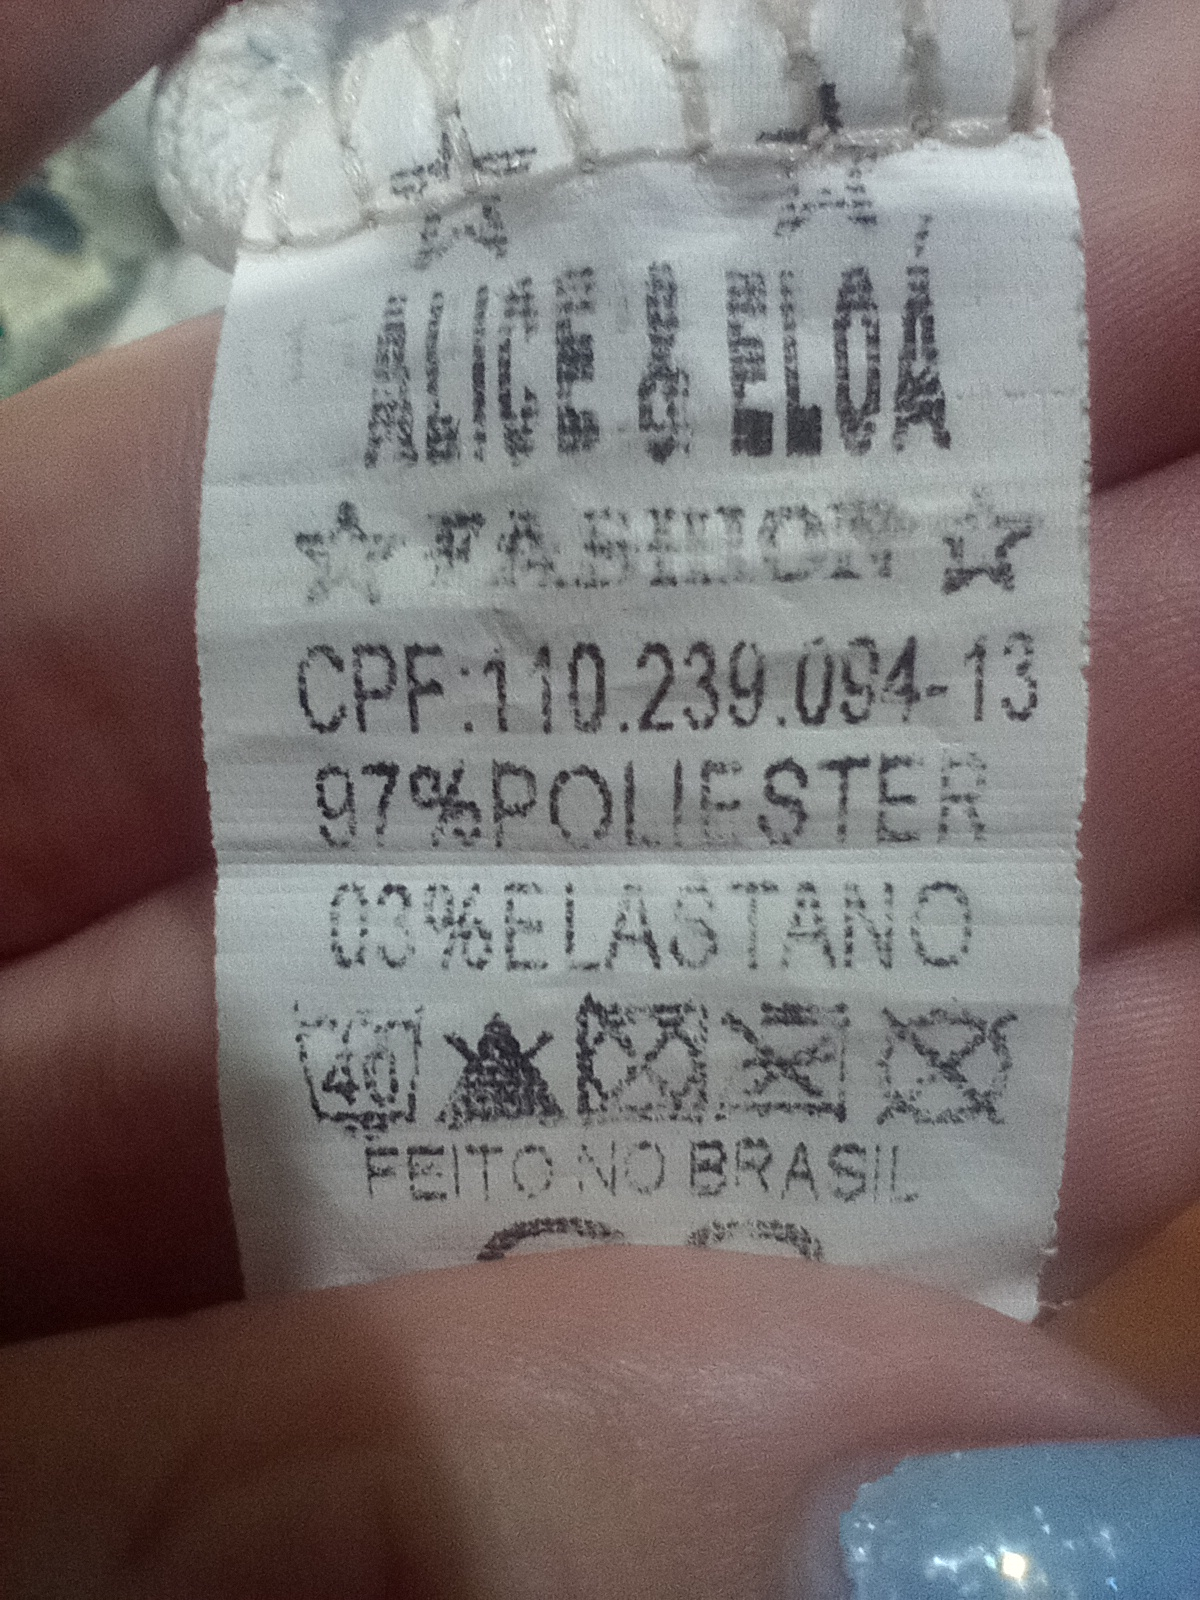
\includegraphics[width=\linewidth, height=4.4cm, keepaspectratio]{imgs/tecido1.jpg}
  \caption{Etiqueta de composição têxtil.}\label{fig:tecido1}
\end{minipage} &
\begin{minipage}{0.30\textwidth}\centering
  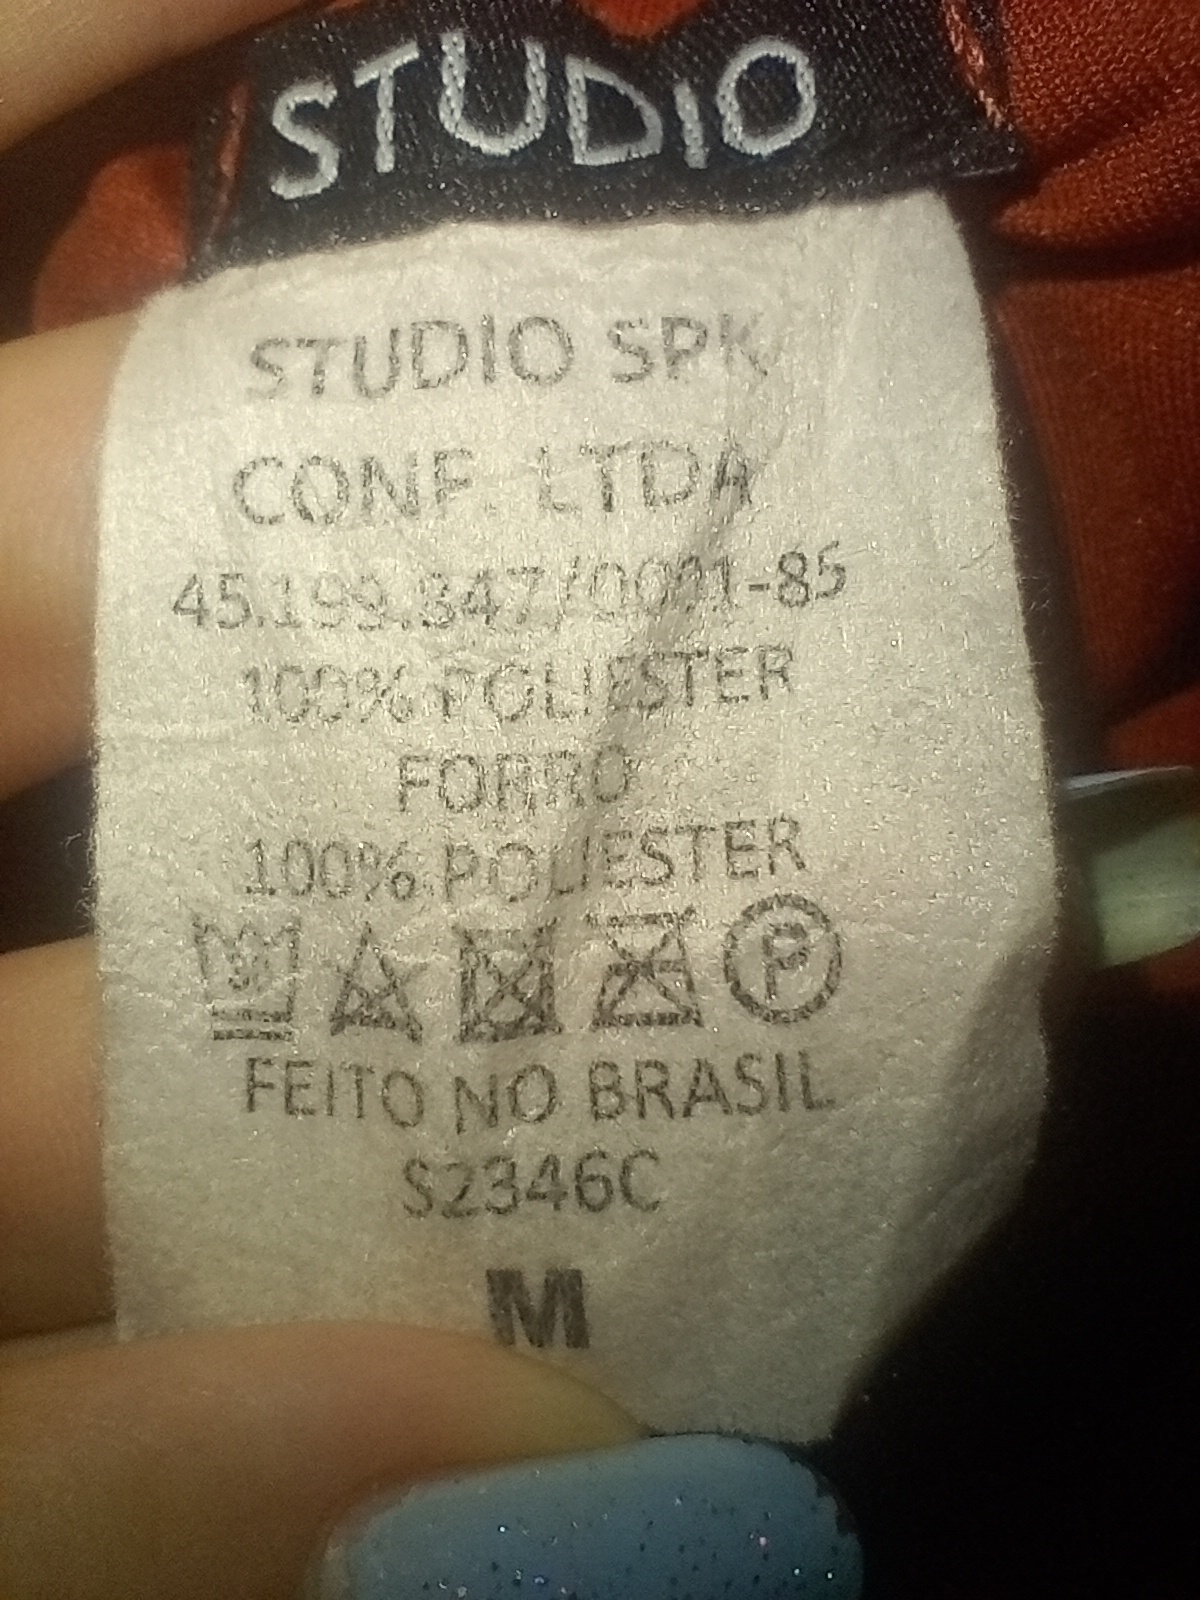
\includegraphics[width=\linewidth, height=4.4cm, keepaspectratio]{imgs/tecido2.jpg}
  \caption{Etiqueta de composição têxtil.}\label{fig:tecido2}
\end{minipage} &
\begin{minipage}{0.30\textwidth}\centering
  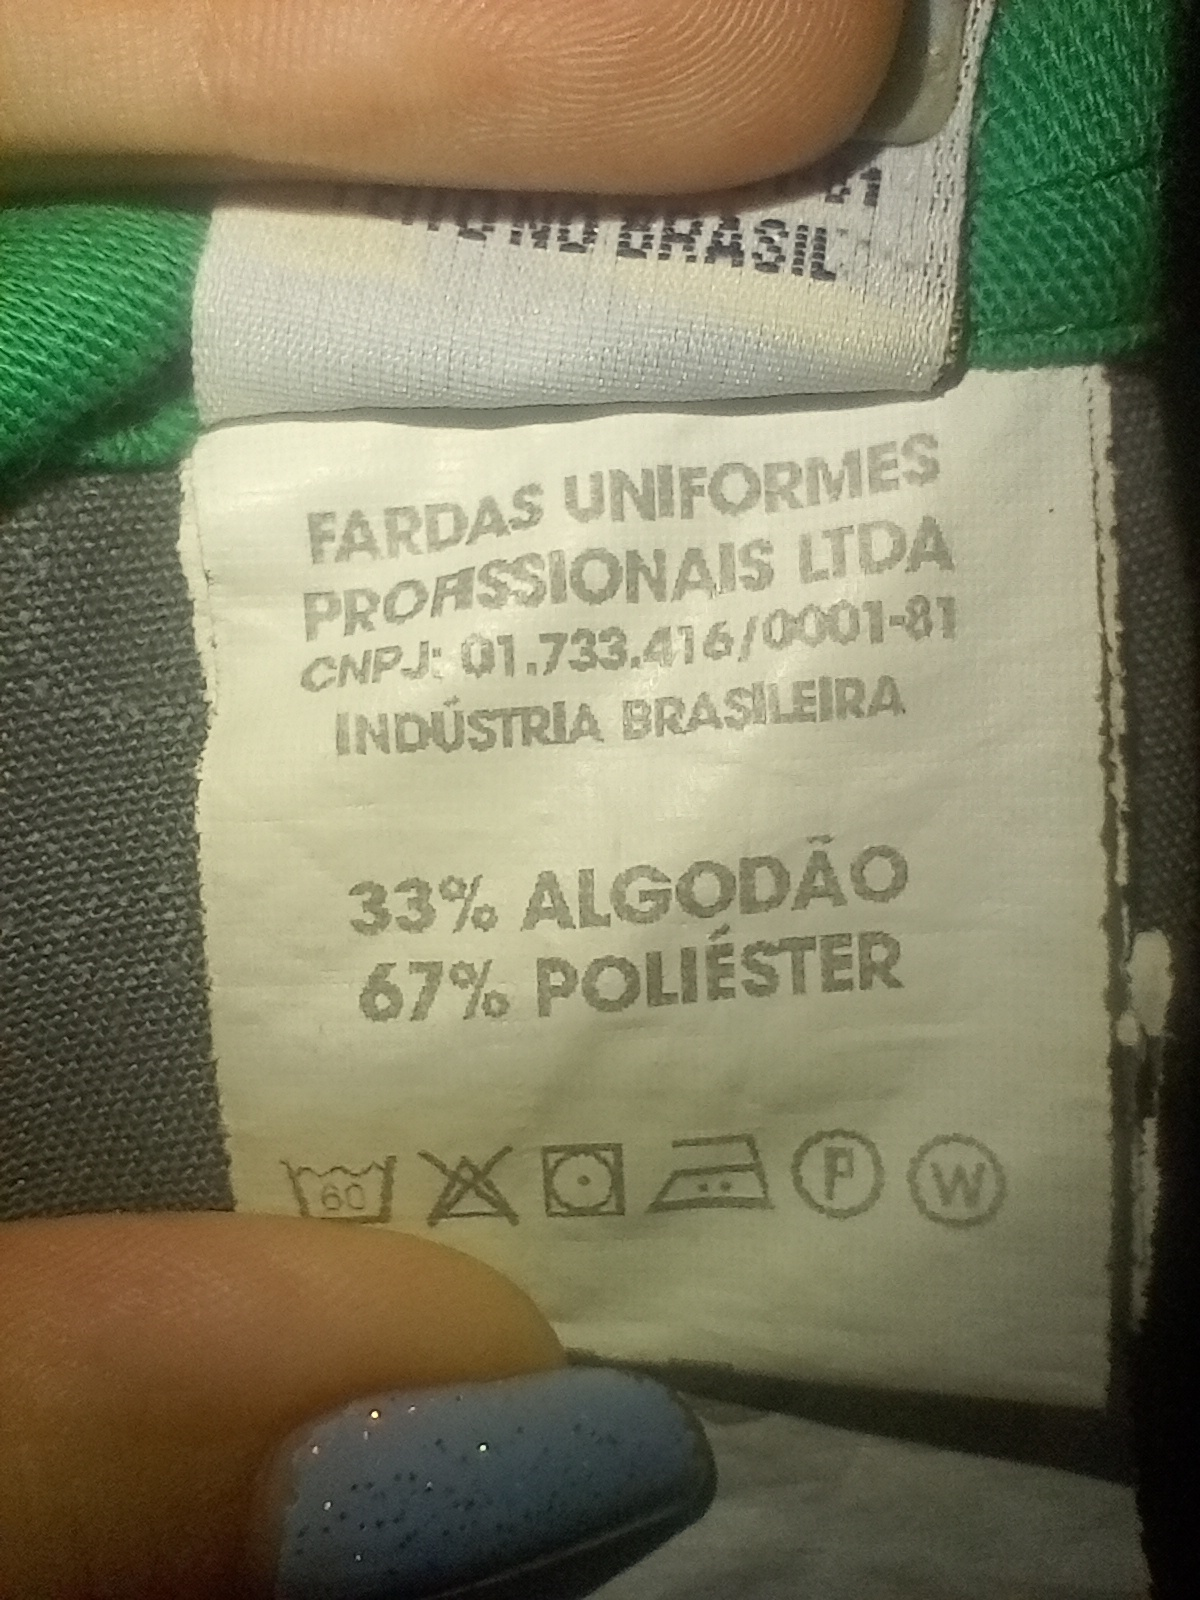
\includegraphics[width=\linewidth, height=4.4cm, keepaspectratio]{imgs/tecido3.jpg}
  \caption{Etiqueta de composição têxtil.}\label{fig:tecido3}
\end{minipage} \\[10pt]
\begin{minipage}{0.30\textwidth}\centering
  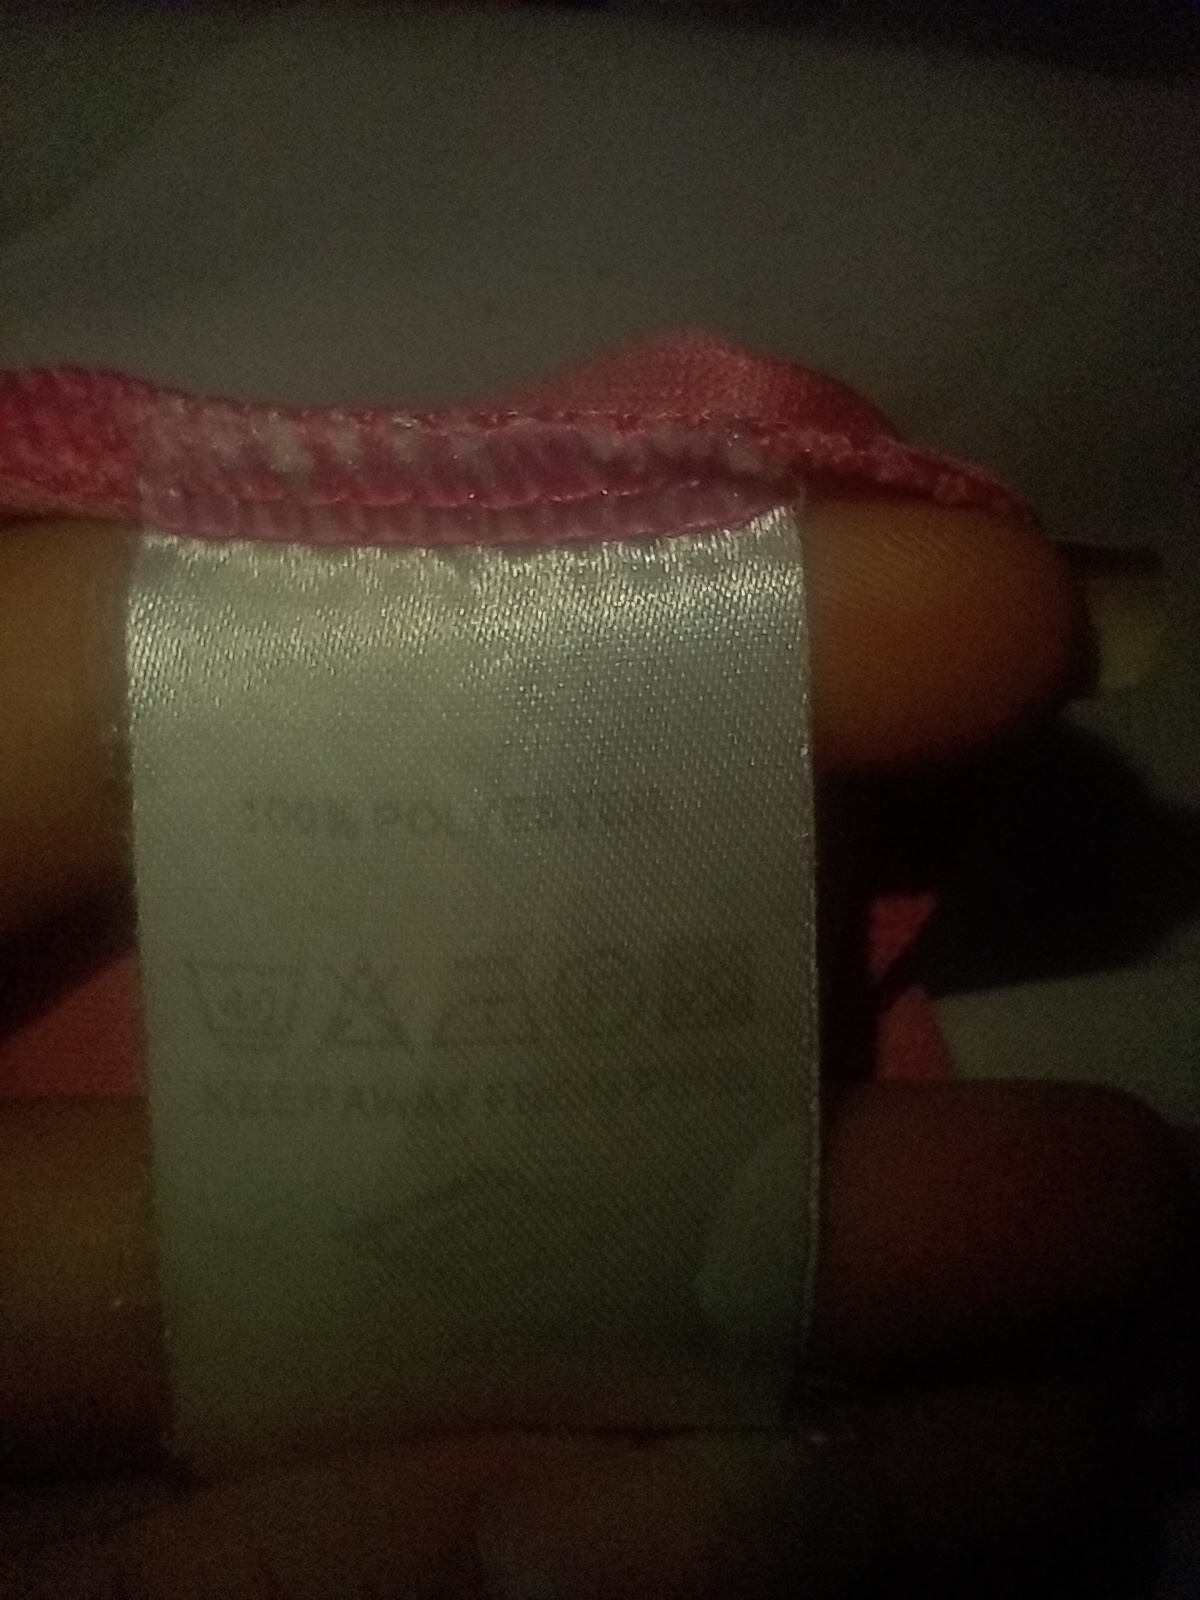
\includegraphics[width=\linewidth, height=4.4cm, keepaspectratio]{imgs/tecido4.jpg}
  \caption{Etiqueta de composição têxtil.}\label{fig:tecido4}
\end{minipage} &
\begin{minipage}{0.30\textwidth}\centering
  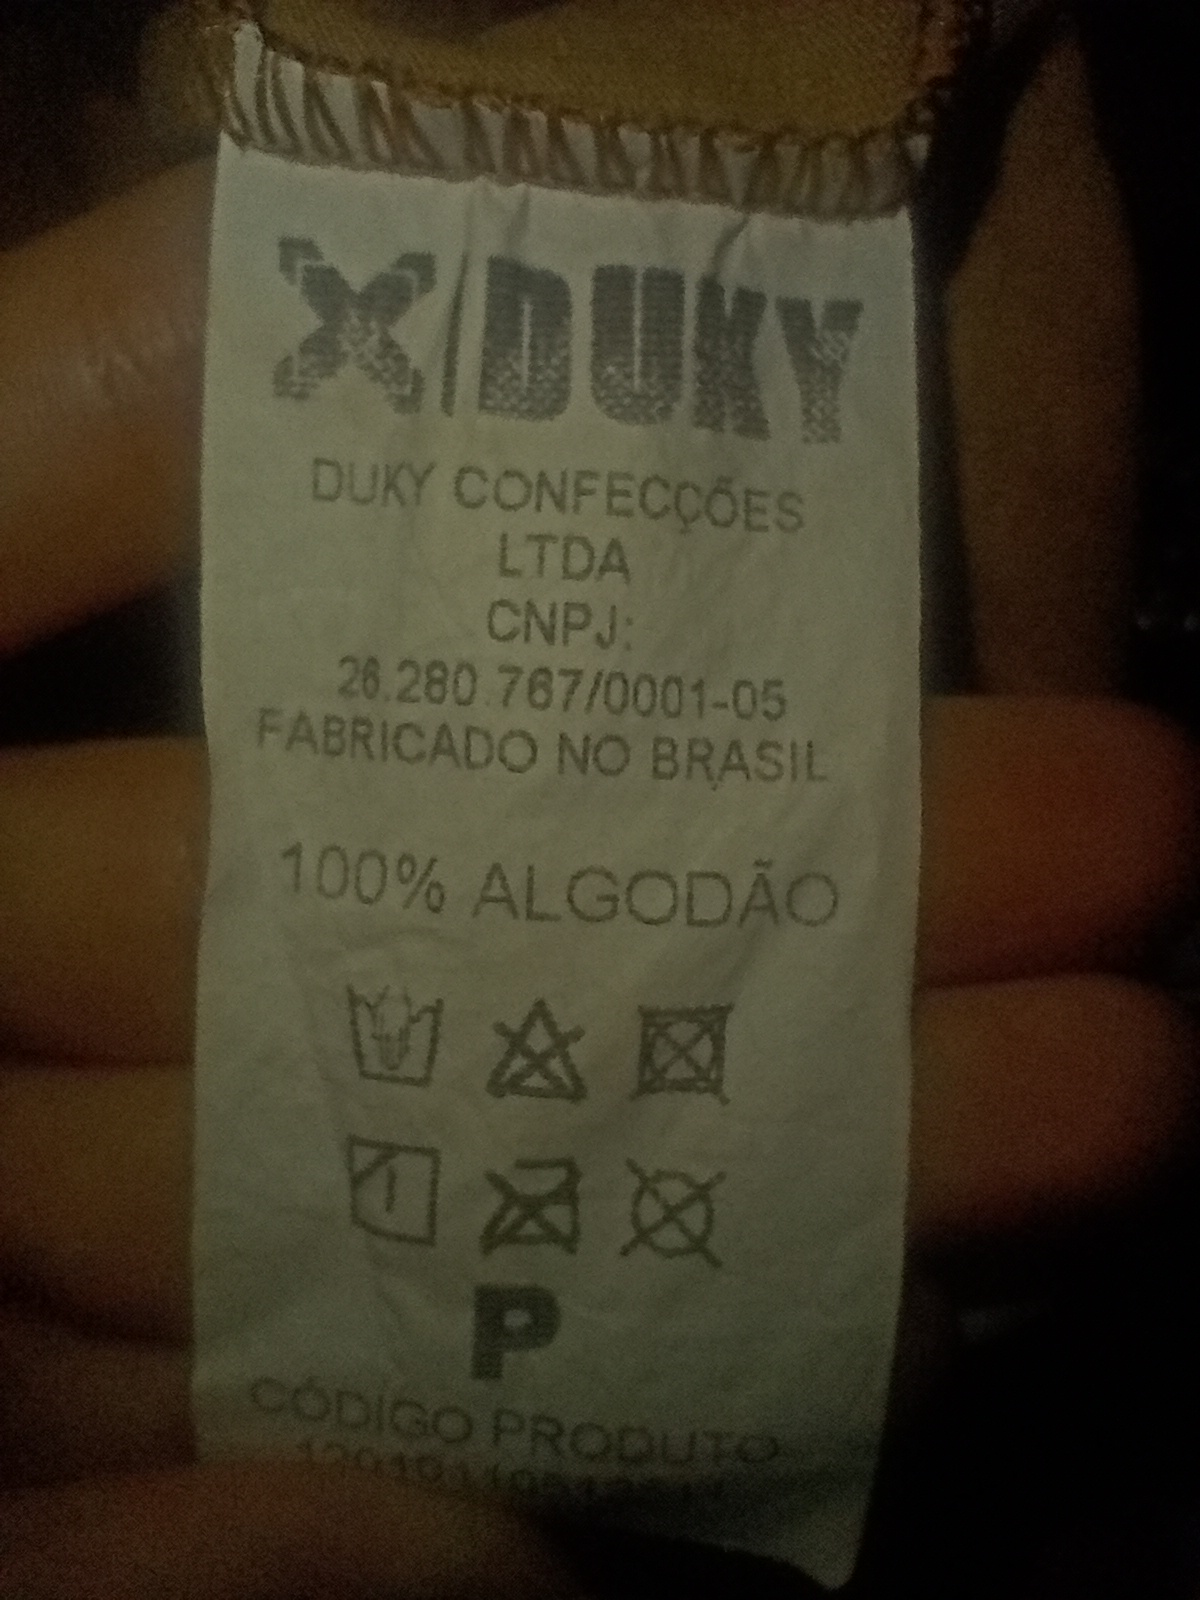
\includegraphics[width=\linewidth, height=4.4cm, keepaspectratio]{imgs/tecido5.jpg}
  \caption{Etiqueta de composição têxtil.}\label{fig:tecido5}
\end{minipage} &
\begin{minipage}{0.30\textwidth}\centering
  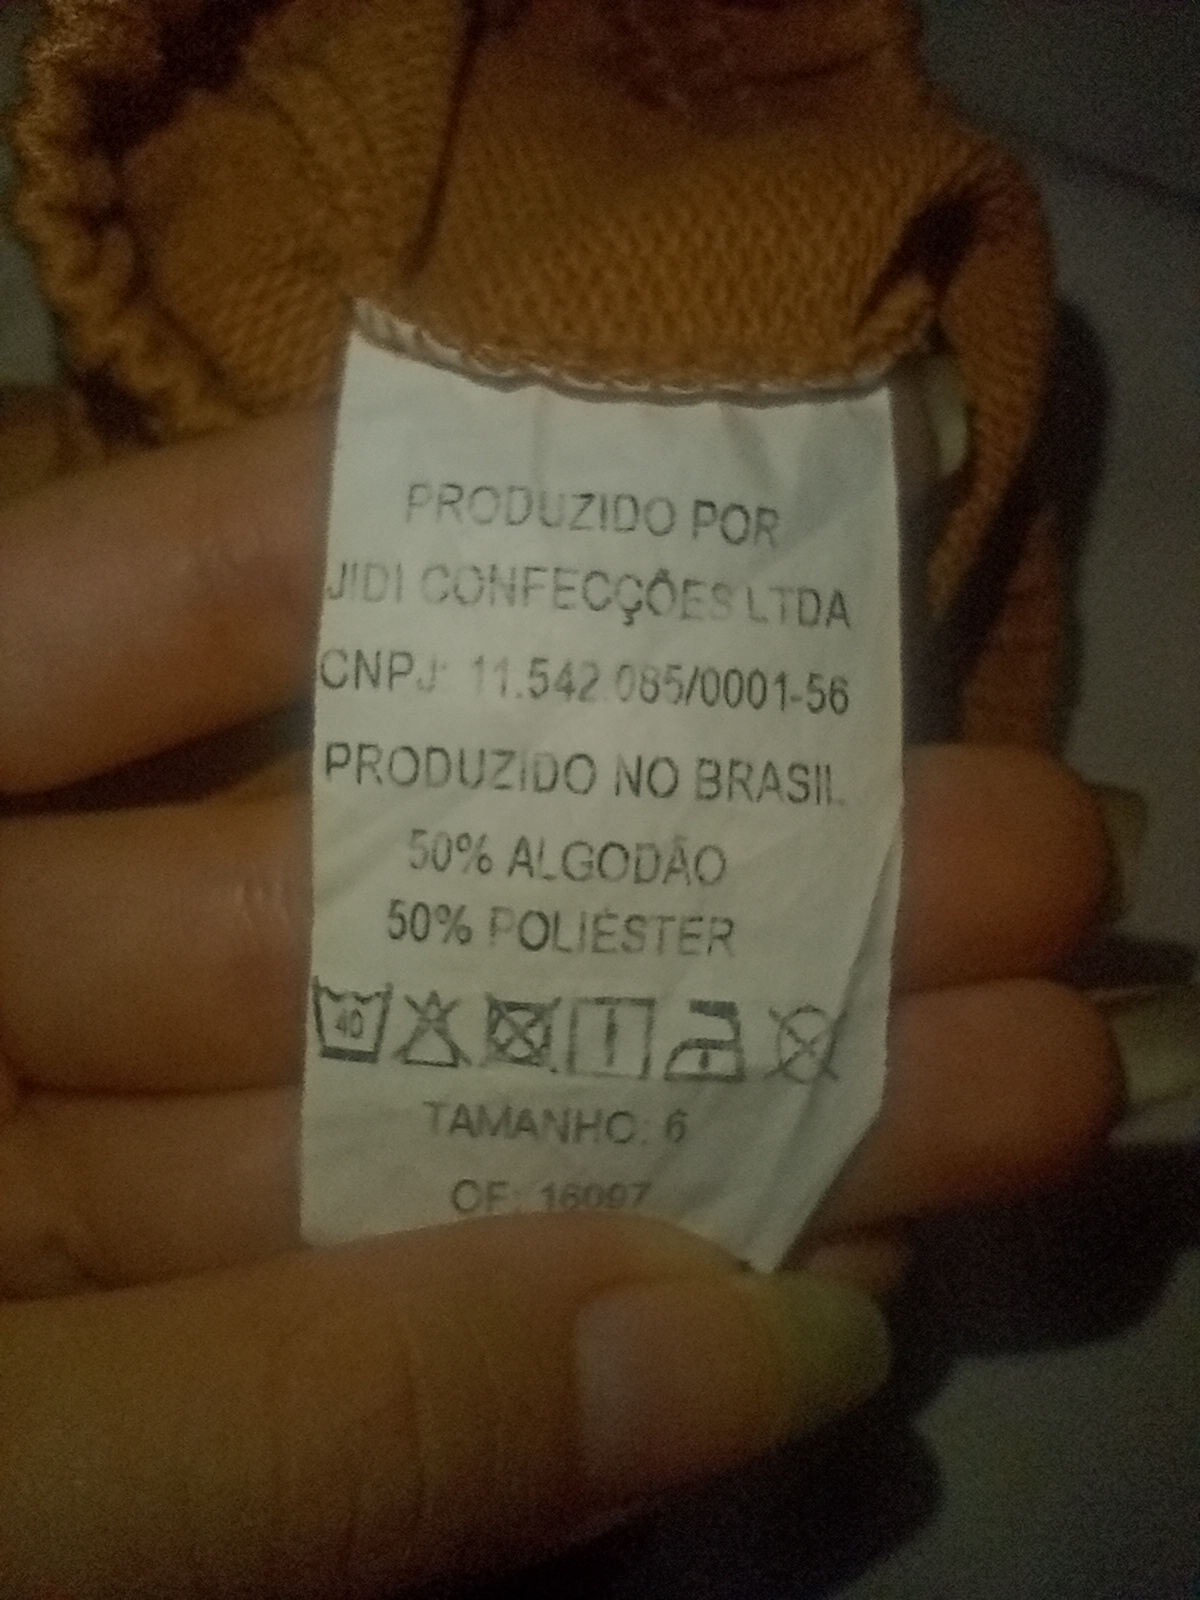
\includegraphics[width=\linewidth, height=4.4cm, keepaspectratio]{imgs/tecido6.jpg}
  \caption{Etiqueta de composição têxtil.}\label{fig:tecido6}
\end{minipage} \\
\end{tabular}
\vspace{6pt}

{\footnotesize\color{slate}Fonte: do autor (2026). Roupas com material 100\% poliéster ou que contém poliéster.}
\end{figure}

Também foi observado que em muitos casos o poliéster é misturado com outros tecidos sintéticos como o elastano, ele não existe na natureza e é derivado do petróleo, sendo composto por polímeros de poliuretano. (o poliuretano é uma corrente de macromoléculas sintéticas criada a partir da reação de compostos orgânicos, cuja estrutura pode ser manipulada para criar desde tecidos elásticos até plásticos de alta resistência.)

Entre vários outros aspectos podemos entender que, tecidos sintéticos liberam micro partículas de plástico que contaminam os oceanos e a cadeia alimentar.

\citacaoDestaque{``A poluição proveniente do plástico é apenas uma parte das ações da sociedade que impactam diretamente o meio ambiente, segundo Green Me (2017), a indústria da moda contribui através das fibras sintéticas que são derivadas do plástico e que colaboram para a poluição dos oceanos. A cada ano a indústria têxtil dispensa entre 40 e 50 mil toneladas de corantes artificiais em fontes de água potável. Esses corantes, a base de benzidina, são altamente cancerígenos e apresentam risco de vida a todos os humanos (LEE, 2011). Por sua grande utilização na indústria têxtil, o poliéster é um dos microplásticos mais encontrados em forma de fibra nos mares e oceanos (NAPPER e THOMPSON, 2016 apud FONTANA, MOSSOTTI e MONTARSOLO, 2020). A origem desses microplásticos é proveniente tanto dos processos de fabricação das fibras sintéticas como da manutenção das peças confeccionadas por meio da lavagem doméstica.''\textsuperscript{7}}{Microplásticos e a indústria do vestuário}

Por fim, o descarte incorreto de tecidos (especialmente os sinteticos) geram em varios locais do mundo um fenomeno chamado ``cemiterio de roupas'' em um artigo da BCC fala um pouco sobre esse tipo de descarte.

\citacaoDestaque{``Caminhões carregados com fardos de roupa usada entram e saem da Zona Franca de Iquique, mais conhecida como Zofri. Este paraíso das compras abriga um imenso parque industrial onde operam mais de mil empresas que comercializam seus produtos isentos de impostos. Seu lugar estratégico no norte do Chile --- a poucos quilômetros do porto do Iquique --- transforma a área em um importante centro comercial para outros países latino-americanos como Argentina, Brasil, Peru e Bolívia.''}{BBC News Brasil --- O cemitério de fast fashion no Atacama}

\begin{figure}[H]
\centering
% >>> A Figura 7 é foto de terceiros (Bernetti/AFP via BBC). Quando tiver o
%     arquivo, salve como imgs/atacama.jpg e troque o bloco abaixo por:
%     \includegraphics[width=0.8\textwidth]{imgs/atacama.jpg}
\setlength{\fboxsep}{0pt}%
\fcolorbox{oliveSoft}{cream}{\parbox[c][5cm][c]{0.8\textwidth}{\centering\color{slate}\small\itshape [ Inserir imagem \textemdash{} Figura 7 ]\\[2pt]Montanha de roupas descartadas no Deserto do Atacama, no Chile.}}
\caption{Montanha de roupas descartadas no Deserto do Atacama, no Chile.}\label{fig:atacama}
{\footnotesize\color{slate}Fonte: Bernetti / AFP via BBC (2022).\textsuperscript{8}}
\end{figure}

\subsection{Formulário}
Pesquisa de campo para saber se o público tem um hábito de reciclar artigos de vestuário e como é a relação deles sobre o ciclo de vida de tais artigos. Ao total são 4 perguntas, tivemos 17 respostas para coletar e analisar dados.

% ---------- GRÁFICO 8 ----------
\begin{figure}[H]
\centering
\caption{Qual é a sua maior dificuldade para reciclar ou descartar roupas que não servem mais? \\ \small Amostra: 17 pessoas que responderam via internet}\label{fig:graf8}
\vspace{4pt}
\begin{tikzpicture}
\pie[radius=2, color={olive, accentYellow, oliveSoft}, text=,
     every only number node/.style={text=white, font=\footnotesize\bfseries}]{66.7, 28.6, 4.8}
\end{tikzpicture}
\vspace{8pt}

\begin{minipage}{0.92\textwidth}\footnotesize
\legendaItem{olive}{\textbf{66,7\%} --- Não conheço pontos de coleta próximos à minha casa}
\legendaItem{accentYellow}{\textbf{28,6\%} --- Falta de tempo para levar as peças a um local específico}
\legendaItem{oliveSoft}{\textbf{4,8\%} --- Não sei quais materiais ou marcas são recicláveis}
\end{minipage}
\end{figure}

% ---------- GRÁFICO 9 ----------
\begin{figure}[H]
\centering
\caption{Com que frequência você avalia o estado das suas roupas para doação ou reciclagem? \\ \small Amostra: 17 pessoas que responderam via internet}\label{fig:graf9}
\vspace{4pt}
\begin{tikzpicture}
\pie[radius=2, color={olive, oliveSoft, accentYellow}, text=,
     every only number node/.style={text=white, font=\footnotesize\bfseries}]{66.7, 28.6, 4.8}
\end{tikzpicture}
\vspace{8pt}

\begin{minipage}{0.92\textwidth}\footnotesize
\legendaItem{olive}{\textbf{66,7\%} --- Raramente (apenas quando o guarda-roupa fica muito cheio)}
\legendaItem{oliveSoft}{\textbf{28,6\%} --- Uma ou duas vezes por ano (trocas de estação)}
\legendaItem{accentYellow}{\textbf{4,8\%} --- Nunca (guardo até ficarem inutilizáveis)}
\end{minipage}
\end{figure}

% ---------- GRÁFICO 10 ----------
\begin{figure}[H]
\centering
\caption{O quanto você se sente satisfeito com as informações que as marcas dão sobre a durabilidade das peças? \\ \small Amostra: 17 pessoas que responderam via internet}\label{fig:graf10}
\vspace{4pt}
\begin{tikzpicture}
\pie[radius=2, color={olive, oliveSoft, accentYellow, slate}, text=,
     every only number node/.style={text=white, font=\footnotesize\bfseries}]{47.6, 19, 19, 14.3}
\end{tikzpicture}
\vspace{8pt}

\begin{minipage}{0.92\textwidth}\footnotesize
\legendaItem{olive}{\textbf{47,6\%} --- Parcialmente satisfeito, mas sinto falta de dados reais de duração}
\legendaItem{oliveSoft}{\textbf{19\%} --- Insatisfeito, as roupas duram bem menos do que o esperado}
\legendaItem{accentYellow}{\textbf{19\%} --- Muito insatisfeito, não encontro informação sobre o ciclo de vida}
\legendaItem{slate}{\textbf{14,3\%} --- Muito satisfeito, as instruções são claras e precisas}
\end{minipage}
\end{figure}

% ---------- GRÁFICO 11 ----------
\begin{figure}[H]
\centering
\caption{O que mais te motivaria a usar um aplicativo para registrar o descarte correto de uma peça? \\ \small Amostra: 17 pessoas que responderam via internet}\label{fig:graf11}
\vspace{4pt}
\begin{tikzpicture}
\pie[radius=2, color={olive, oliveSoft, accentYellow, slate}, text=,
     every only number node/.style={text=white, font=\footnotesize\bfseries}]{52.4, 23.8, 19, 4.8}
\end{tikzpicture}
\vspace{8pt}

\begin{minipage}{0.92\textwidth}\footnotesize
\legendaItem{olive}{\textbf{52,4\%} --- Ter a certeza de que a roupa terá um destino ambientalmente correto}
\legendaItem{oliveSoft}{\textbf{23,8\%} --- Receber dicas personalizadas de como cuidar melhor das minhas roupas}
\legendaItem{accentYellow}{\textbf{19\%} --- Receber cupons de desconto em marcas parceiras}
\legendaItem{slate}{\textbf{4,8\%} --- Ganhar selos de sustentabilidade e subir em um ranking de amigos}
\end{minipage}
\end{figure}

\correcao{Conferir os dados: as Figuras~\ref{fig:graf8} e \ref{fig:graf9} apresentam exatamente a mesma distribuição (66,7\% / 28,6\% / 4,8\%) para perguntas diferentes. Verificar no Google Forms se os números das duas perguntas estão corretos ou se houve duplicação ao transcrever as respostas.}

\subsection*{Diagnóstico do Formulário}
Os resultados da pesquisa revelam que o principal gargalo no ciclo de consumo e descarte de vestuário é de natureza logística, afetando diretamente 94,1\% dos entrevistados devido à falta de tempo ou ao desconhecimento sobre onde entregar as peças; essa barreira prática gera um efeito dominó de desinteresse fazendo com que 70,6\% das pessoas realizem o descarte de forma rara e reativa, apenas quando o guarda-roupa fica completamente lotado. Ao mesmo tempo que esse desafio estrutural existe, constata-se um cenário de insatisfação quase total com a postura das empresas, onde só 11,8\% consideram a comunicação das marcas eficiente, evidenciando uma forte demanda por dados reais sobre a durabilidade e a qualidade dos tecidos. Diante disso, o público sinaliza que dispensa campanhas puramente motivacionais, exigindo, em vez disso, transparência absoluta sobre o destino final das roupas descartadas e o fornecimento de guias práticos de conservação para que possam cuidar melhor de suas peças e prolongar sua vida útil.

% ============================================================================
%  5. DEFINIÇÃO
% ============================================================================
\novaSecao{Definição}

A etapa de Definição é o momento do Design Thinking em que sintetizamos tudo o que foi descoberto na Imersão para delimitar, com clareza, qual problema vamos resolver. Depois de divergir \textemdash{} coletando dados na Pesquisa Desk, na Observação e no Formulário \textemdash{}, aqui nós convergimos: organizamos os achados em ferramentas visuais (enunciado do problema, persona, mapa de empatia e jornada do usuário) que transformam informação dispersa em um retrato concreto de quem é afetado e do que essa pessoa precisa. É essa definição que orienta a fase seguinte, a Ideação.

\subsection{Enunciado do Problema}

A partir da síntese dos dados da Imersão, o problema central do projeto foi definido no seguinte enunciado:

\begin{citacaoBox}
Pessoas que consomem vestuário com frequência precisam de uma forma simples e confiável de descartar e reciclar suas roupas, porque hoje faltam pontos de coleta acessíveis e informação sobre o destino correto das peças \textemdash{} o que leva ao acúmulo e ao descarte incorreto.
\end{citacaoBox}

\correcao{Enunciado proposto a partir dos dados do formulário (gargalo logístico). Conferir se ele reflete a dor principal apontada pela persona; se a persona indicar outra prioridade, ajustar a frase para casar com ela.}

\subsection{Persona}

A Figura~\ref{fig:persona} apresenta o painel visual da persona construída no Figma, consolidando os principais atributos identificados.

\begin{figure}[H]
    \centering
    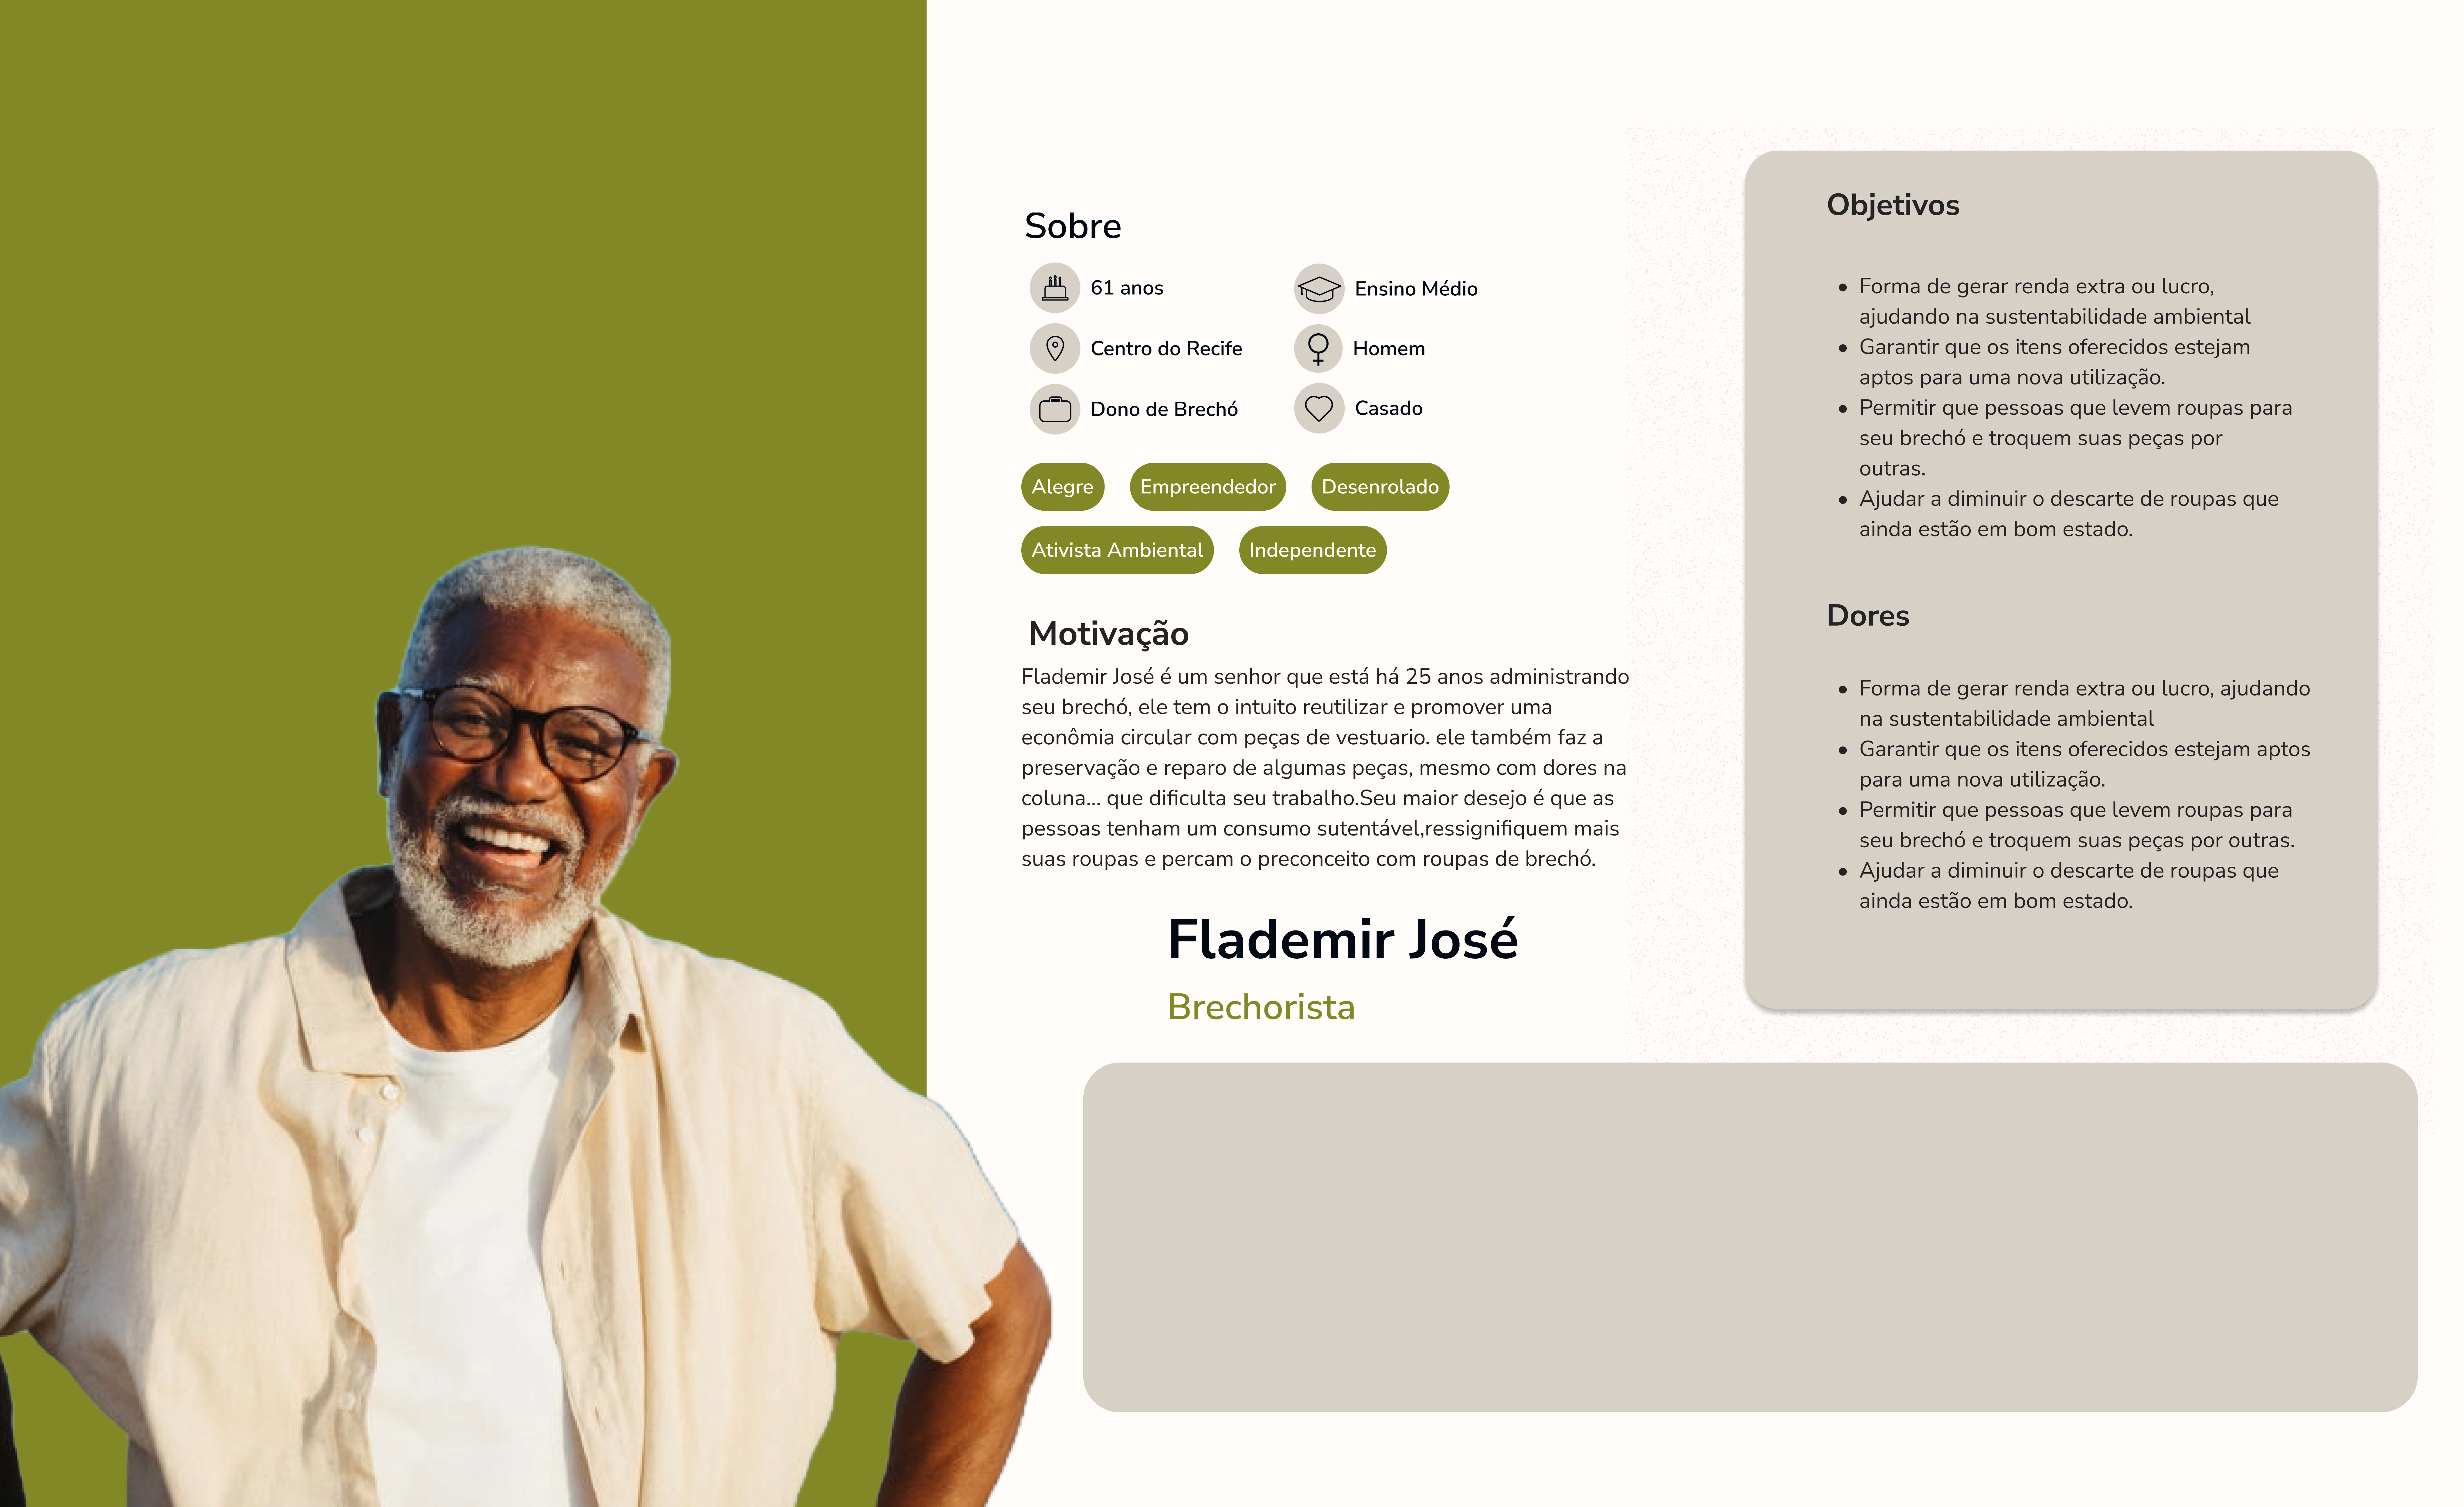
\includegraphics[width=\textwidth]{imgs/persona-fladmir.png}
    \caption{Painel visual da Persona}
    \label{fig:persona}
\end{figure}

\subsection{Mapa de Empatia}

O Mapa de Empatia foi construído como ferramenta de síntese qualitativa, organizado em sete dimensões que aprofundam a compreensão da experiência da persona para além dos dados numéricos do formulário.

A Figura~\ref{fig:empatia} apresenta o Mapa de Empatia visual elaborado no Figma, estruturado conforme os sete quadrantes da ferramenta.

\begin{figure}[H]
    \centering
    \includegraphics[width=\textwidth]{imgs/mapa-empatia-fladmir.png}
    \caption{Mapa de Empatia}
    \label{fig:empatia}
\end{figure}

\subsection{Jornada do Usuário}

A Figura~\ref{fig:jornada} apresenta a representação visual da Jornada do Usuário elaborada no Figma.

\begin{figure}[H]
    \centering
    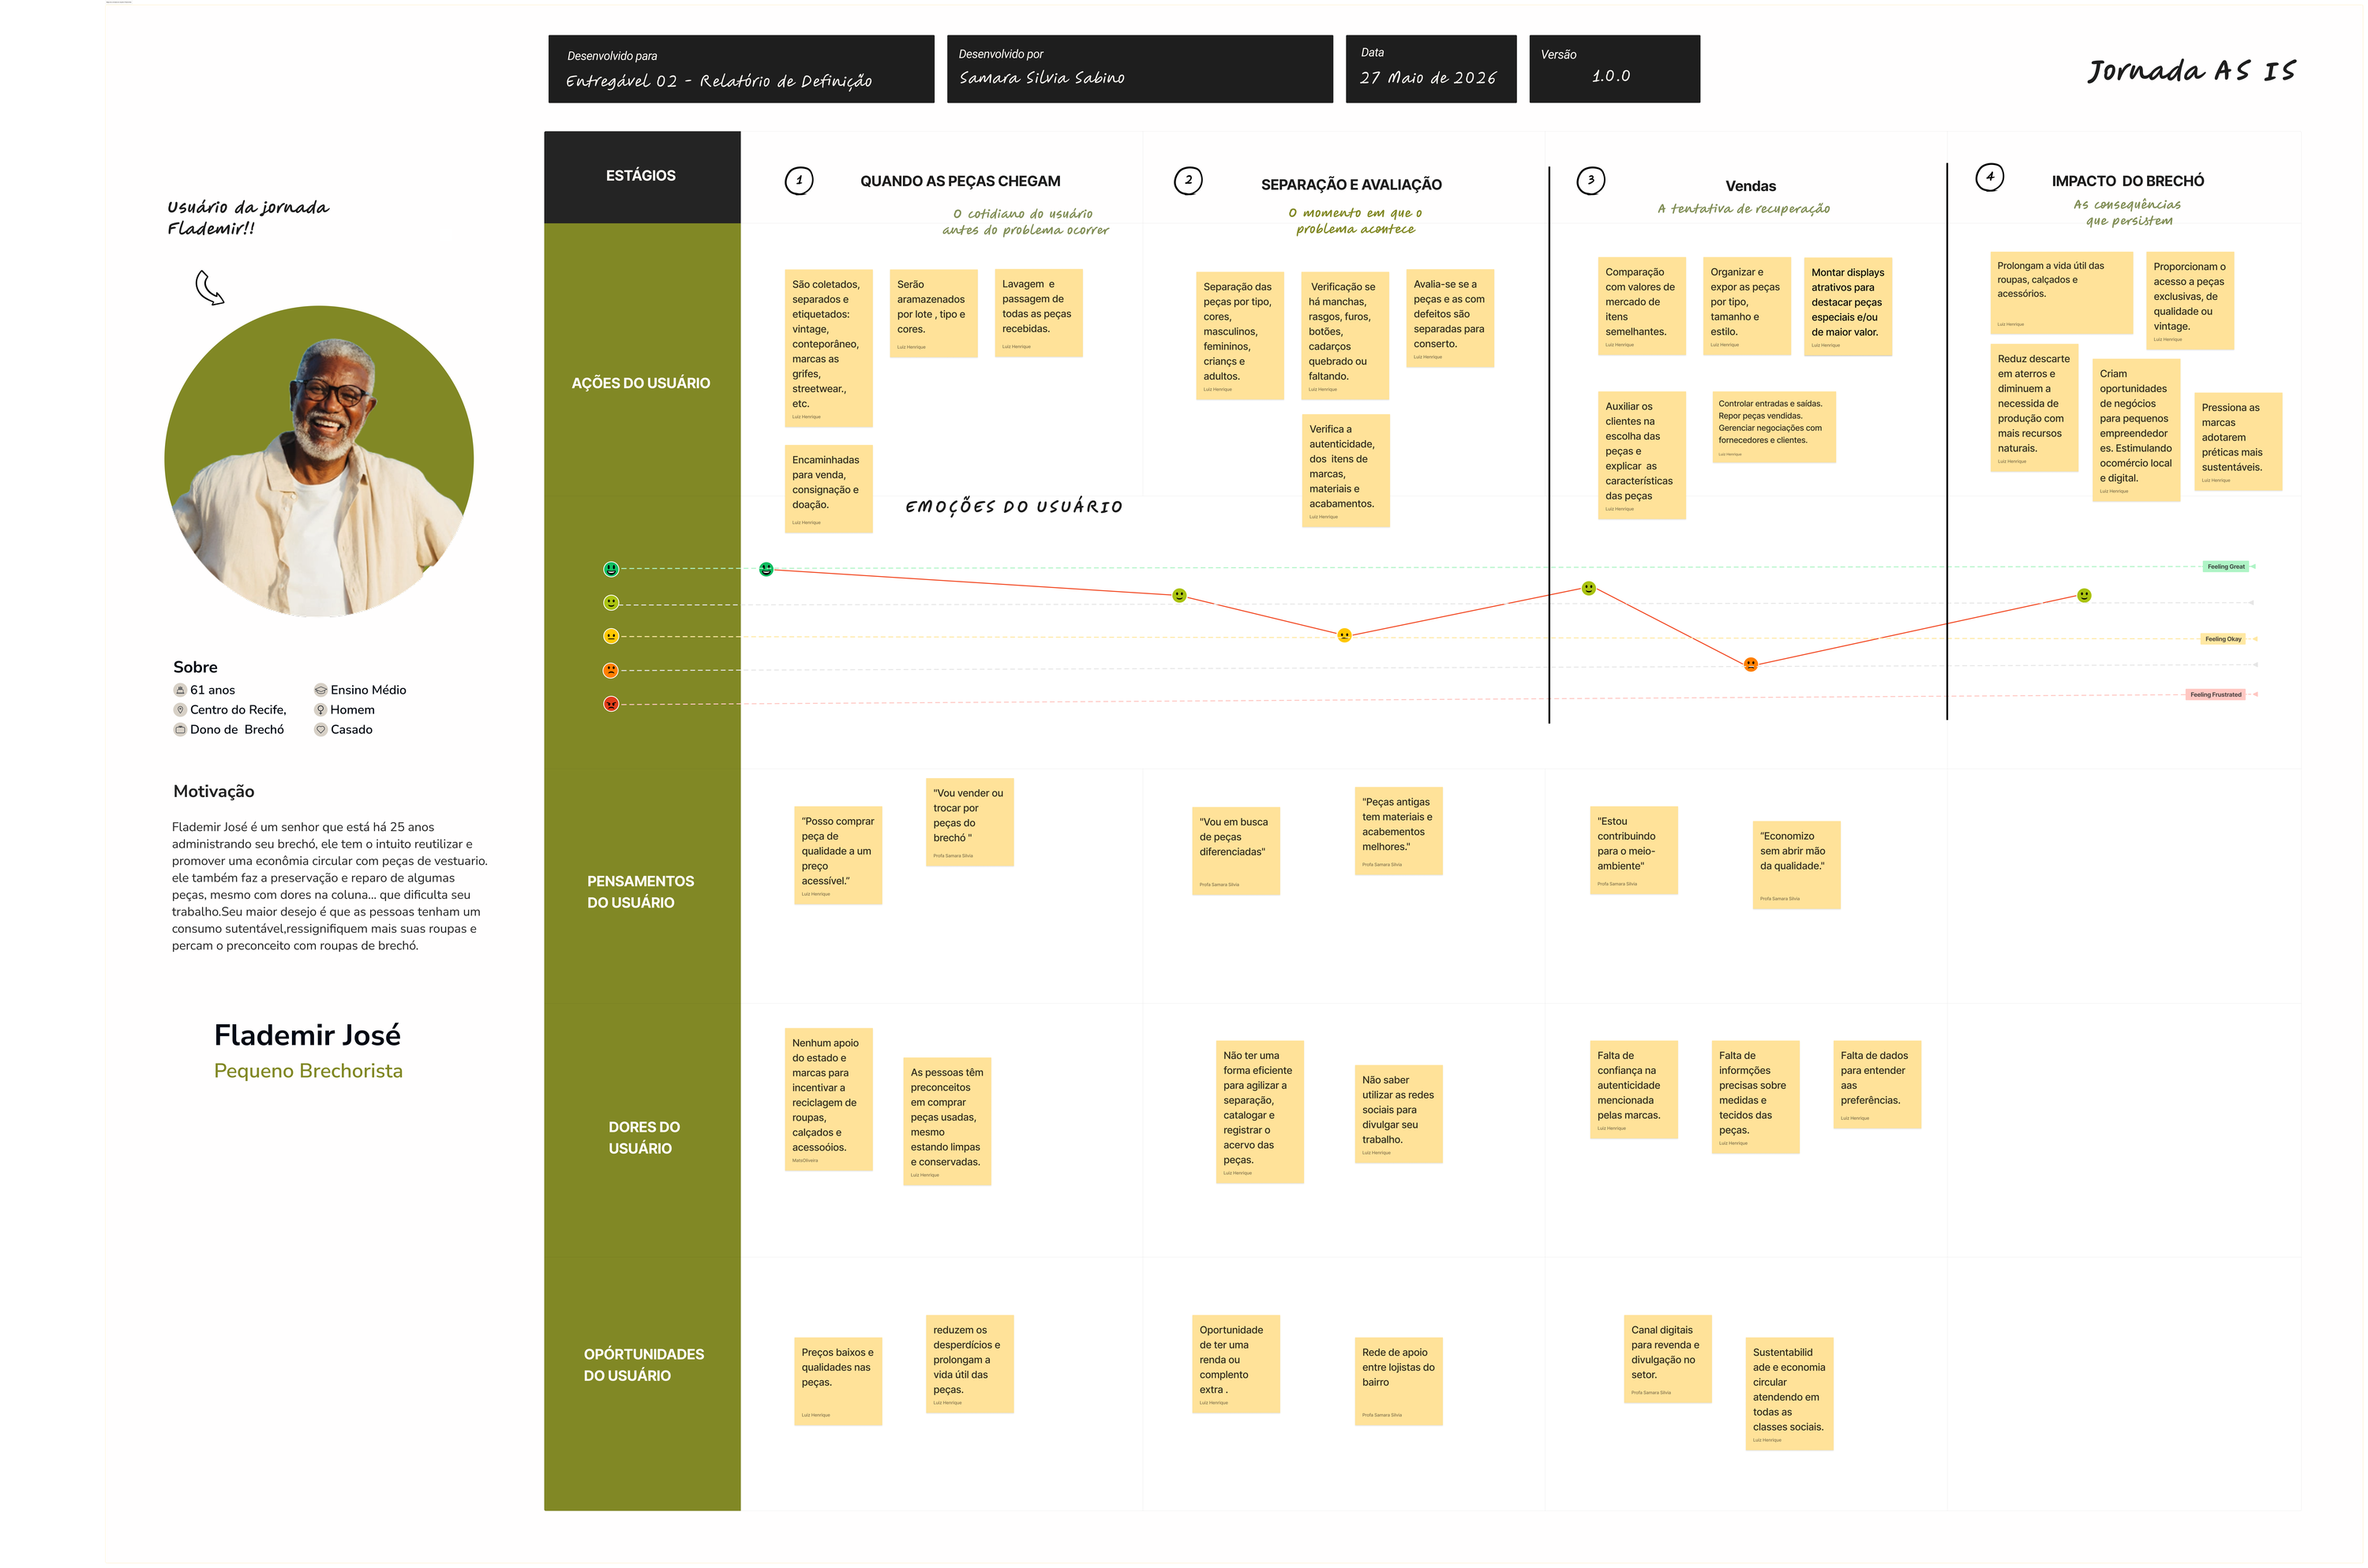
\includegraphics[width=\textwidth]{imgs/jornada-usuario-fladmir.png}
    \caption{Mapa da Jornada do Usuário}
    \label{fig:jornada}
\end{figure}

% ============================================================================
%  6. REFERÊNCIAS
% ============================================================================
\novaSecao{Referências}

\noindent\textit{Todas as pesquisas e artigos adicionados foram publicados no período de 2019 há 2024.}

\vspace{10pt}
\newcommand{\refnum}[1]{\textcolor{oliveDeep}{\sffamily\bfseries[#1]}\ }
\setlength{\parskip}{10pt}

\refnum{1, 4} SANTOS, Vanessa Faria dos. \textbf{Reciclagem têxtil: algodão e poliéster}. Orientador: José Ângelo Bortoloto. 2020. Monografia (Trabalho de Conclusão de Curso) --- Centro Paula Souza, [S. l.], 2020. Disponível em: \url{https://ric.cps.sp.gov.br/handle/123456789/6270}. Acesso em: 21 maio 2026.

\refnum{2, 6} REZENDE, Isabela Yankous Vale Santos; LOPES, Camila Santos Doubek. \textbf{Greenwashing e impacto ambiental na indústria têxtil: um estudo de caso}. Projetica, Londrina, v. 10, n. 2, p. 187--208, 2019. DOI: 10.5433/2236-2207.2019v10n2p187. Disponível em: \url{https://ojs.uel.br/revistas/uel/index.php/projetica/article/view/32767}. Acesso em: 21 maio 2026.

\refnum{3} BRASIL. Controladoria-Geral da União. \textbf{Design Thinking}. Portal Gov.br, [202-?]. Disponível em: \url{https://www.gov.br/ouvidorias/pt-br/governanca-de-servicos/ferramentas/design-thinking}. Acesso em: 21 maio 2026.

\refnum{5} NIINIMÄKI, Kirsi et al. \textbf{The environmental price of fast fashion}. Nature Reviews Earth \& Environment, [S. l.], v. 1, n. 4, p. 189--200, 2020. DOI: \url{https://doi.org/10.1038/s43017-020-0039-9}. Disponível em: \url{https://www.nature.com/articles/s43017-020-0039-9}. Acesso em: 21 maio 2026.

\refnum{7} DEMINSKI, Carla Carolina Deola. \textbf{Microplásticos e a indústria do vestuário: uma revisão}. 2021. Trabalho de Conclusão de Curso (Tecnologia em Design de Moda) --- Instituto Federal de Educação, Ciência e Tecnologia do Rio Grande do Sul, Erechim, 2021. Disponível em: \url{https://dspace.ifrs.edu.br/xmlui/handle/123456789/1740}. Acesso em: 24 maio 2026.

\refnum{8} BERNETTI, Martin. \textbf{Montanha de roupas descartadas no Deserto do Atacama, no Chile}. 2022. 1 fotografia. Agence France-Presse. In: BBC NEWS BRASIL. O cemitério de `fast fashion' no deserto do Atacama. Londres, 25 jan. 2022. Disponível em: \url{https://www.bbc.com/portuguese/internacional-60144656}. Acesso em: 24 maio 2026.

\vspace{6pt}
\noindent{\sffamily\bfseries\color{oliveDeep}\small Material autoral \textemdash{} entrega da Definição}
\vspace{2pt}

\refnum{9} GRUPO 02 (Curso Técnico em Desenvolvimento de Sistemas, ETE Cícero Dias). \textbf{REVESTU \textemdash{} Definição: moda sustentável}: persona, mapa de empatia e jornada do usuário. Recife, 2026. Projeto de design elaborado no Figma. Disponível em: \url{https://www.figma.com/design/PuwjNqwnNExc5uRhbNMHH0/Grupo-02-Definicao-Moda-Sustentavel}. Acesso em: 10 jun. 2026.

\end{document}